%definira klasu dokumenta 
\documentclass[12pt]{report} 

%prostor izmedu naredbi \documentclass i \begin{document} se zove uvod. U njemu se nalaze naredbe koje se odnose na cijeli dokument

%osnovni LaTex ne može riješiti sve probleme, pa se koriste različiti paketi koji olakšavaju izradu željenog dokumenta
\usepackage[croatian]{babel} 
\usepackage{amssymb}
\usepackage{amsmath}
\usepackage{txfonts}
\usepackage{mathdots}
\usepackage{titlesec}
\usepackage{array}
\usepackage{lastpage}
\usepackage{etoolbox}
\usepackage{tabularray}
\usepackage{color, colortbl}
\usepackage{adjustbox}
\usepackage{geometry}
\usepackage[classicReIm]{kpfonts}
\usepackage{hyperref}
\usepackage{fancyhdr}

\usepackage{float}
\usepackage{setspace}
\restylefloat{table}


\patchcmd{\chapter}{\thispagestyle{plain}}{\thispagestyle{fancy}}{}{} %redefiniranje stila stranice u paketu fancyhdr

%oblik naslova poglavlja
\titleformat{\chapter}{\normalfont\huge\bfseries}{\thechapter.}{20pt}{\Huge}
\titlespacing{\chapter}{0pt}{0pt}{40pt}


\linespread{1.3} %razmak između redaka

\geometry{a4paper, left=1in, top=1in,}  %oblik stranice

\hypersetup{ colorlinks, citecolor=black, filecolor=black, linkcolor=black,	urlcolor=black }   %izgled poveznice


%prored smanjen između redaka u nabrajanjima i popisima
\newenvironment{packed_enum}{
	\begin{enumerate}
		\setlength{\itemsep}{0pt}
		\setlength{\parskip}{0pt}
		\setlength{\parsep}{0pt}
	}{\end{enumerate}}

\newenvironment{packed_item}{
	\begin{itemize}
		\setlength{\itemsep}{0pt}
		\setlength{\parskip}{0pt}
		\setlength{\parsep}{0pt}
	}{\end{itemize}}




%boja za privatni i udaljeni kljuc u tablicama
\definecolor{LightBlue}{rgb}{0.9,0.9,1}
\definecolor{LightGreen}{rgb}{0.9,1,0.9}

%Promjena teksta za dugačke tablice
\DefTblrTemplate{contfoot-text}{normal}{Nastavljeno na idućoj stranici}
\SetTblrTemplate{contfoot-text}{normal}
\DefTblrTemplate{conthead-text}{normal}{(Nastavljeno)}
\SetTblrTemplate{conthead-text}{normal}
\DefTblrTemplate{middlehead,lasthead}{normal}{Nastavljeno od prethodne stranice}
\SetTblrTemplate{middlehead,lasthead}{normal}

%podesavanje zaglavlja i podnožja

\pagestyle{fancy}
\lhead{Programsko inženjerstvo}
\rhead{Wild Track}
\lfoot{Aristos}
\cfoot{stranica \thepage/\pageref{LastPage}}
\rfoot{\today}
\renewcommand{\headrulewidth}{0.2pt}
\renewcommand{\footrulewidth}{0.2pt}


\begin{document} 
	
	
	
	\begin{titlepage}
		\begin{center}
			\vspace*{\stretch{1.0}} %u kombinaciji s ostalim \vspace naredbama definira razmak između redaka teksta
			\LARGE Programsko inženjerstvo\\
			\large Ak. god. 2023./2024.\\
			
			\vspace*{\stretch{3.0}}
			
			\huge Wild Track\\
			\Large Dokumentacija, Rev. 1.\\
			
			\vspace*{\stretch{12.0}}
			\normalsize
			Grupa: \textit{Aristos}\\
			Voditelj: \textit{Josipa Udovičić}\\
			
			
			\vspace*{\stretch{1.0}}
			Datum predaje: \textit{17. studenog 2023.}\\
	
			\vspace*{\stretch{4.0}}
			
			Nastavnik: \textit{Hrvoje Nuić}\\
		
		\end{center}

	
	\end{titlepage}

	
	\tableofcontents


	\chapter{Dnevnik promjena dokumentacije}
		
		\textbf{\textit{Kontinuirano osvježavanje}}\\
				
		
		\begin{longtblr}[
				label=none
			]{
				width = \textwidth, 
				colspec={|X[2]|X[13]|X[3]|X[3]|}, 
				rowhead = 1
			}
			\hline
			\textbf{Rev.}	& \textbf{Opis promjene/dodatka} & \textbf{Autori} & \textbf{Datum}\\[3pt] \hline
			0.1 & Napravljen predložak.	& * & 22.08.2013. 		\\[3pt] \hline 
			0.2	& Dopisane upute za povijest dokumentacije.\newline Dodane reference. & * & 24.08.2013. 	\\[3pt] \hline 
			0.5 & Dodan \textit{Use Case} dijagram i jedan sekvencijski dijagram, funkcionalni i nefunkcionalni zahtjevi i dodatak A & * & 25.08.2013. \\[3pt] \hline 
			0.6 & Arhitektura i dizajn sustava, algoritmi i strukture podataka & * & 26.08.2013. \\[3pt] \hline 
			0.8 & Povijest rada i trenutni status implementacije,\newline Zaključci i plan daljnjeg rada & * & 28.08.2013. \\[3pt] \hline 
			0.9 & Opisi obrazaca uporabe & * & 07.09.2013. \\[3pt] \hline 
			0.10 & Preveden uvod & * & 08.09.2013. \\[3pt] \hline 
			0.11 & Sekvencijski dijagrami & * & 09.09.2013. \\[3pt] \hline 
			0.12.1 & Započeo dijagrame razreda & * & 10.09.2013. \\[3pt] \hline 
			0.12.2 & Nastavak dijagrama razreda & * & 11.09.2013. \\[3pt] \hline 
			\textbf{1.0} & Verzija samo s bitnim dijelovima za 1. ciklus & * & 11.09.2013. \\[3pt] \hline 
			1.1 & Uređivanje teksta -- funkcionalni i nefunkcionalni zahtjevi & * \newline * & 14.09.2013. \\[3pt] \hline 
			1.2 & Manje izmjene:Timer - Brojilo vremena & * & 15.09.2013. \\[3pt] \hline 
			1.3 & Popravljeni dijagrami obrazaca uporabe & * & 15.09.2013. \\[3pt] \hline 
			1.5 & Generalna revizija strukture dokumenta & * & 19.09.2013. \\[3pt] \hline 
			1.5.1 & Manja revizija (dijagram razmještaja) & * & 20.09.2013. \\[3pt] \hline 
			\textbf{2.0} & Konačni tekst predloška dokumentacije  & * & 28.09.2013. \\[3pt] \hline 
			&  &  & \\[3pt] \hline	
		\end{longtblr}
	
	
		\textit{Moraju postojati glavne revizije dokumenata 1.0 i 2.0 na kraju prvog i drugog ciklusa. Između tih revizija mogu postojati manje revizije već prema tome kako se dokument bude nadopunjavao. Očekuje se da nakon svake značajnije promjene (dodatka, izmjene, uklanjanja dijelova teksta i popratnih grafičkih sadržaja) dokumenta se to zabilježi kao revizija. Npr., revizije unutar prvog ciklusa će imati oznake 0.1, 0.2, …, 0.9, 0.10, 0.11.. sve do konačne revizije prvog ciklusa 1.0. U drugom ciklusu se nastavlja s revizijama 1.1, 1.2, itd.}
	\chapter{Opis projektnog zadatka}
		
		\textbf{\textit{dio 1. revizije}}\\
		
		\textit{Na osnovi projektnog zadatka detaljno opisati korisničke zahtjeve. Što jasnije opisati cilj projektnog zadatka, razraditi problematiku zadatka, dodati nove aspekte problema i potencijalnih rješenja. Očekuje se minimalno 3, a poželjno 4-5 stranica opisa.	Teme koje treba dodatno razraditi u ovom poglavlju su:}
		\begin{packed_item}
			\item \textit{potencijalna korist ovog projekta}
			\item \textit{postojeća slična rješenja (istražiti i ukratko opisati razlike u odnosu na zadani zadatak). Dodajte slike koja predočavaju slična rješenja.}
			\item \textit{skup korisnika koji bi mogao biti zainteresiran za ostvareno rješenje.}
			\item \textit{mogućnost prilagodbe rješenja }
			\item \textit{opseg projektnog zadatka}
			\item \textit{moguće nadogradnje projektnog zadatka}
		\end{packed_item}
		
		\textit{Za pomoć pogledati reference navedene u poglavlju „Popis literature“, a po potrebi konzultirati sadržaj na internetu koji nudi dobre smjernice u tom pogledu.}
		\eject
		
		\section{Primjeri u \LaTeX u}
		
		\textit{Ovo potpoglavlje izbrisati.}\\

		U nastavku se nalaze različiti primjeri kako koristiti osnovne funkcionalnosti \LaTeX a koje su potrebne za izradu dokumentacije. Za dodatnu pomoć obratiti se asistentu na projektu ili potražiti upute na sljedećim web sjedištima:
		\begin{itemize}
			\item Upute za izradu diplomskog rada u \LaTeX u - \url{https://www.fer.unizg.hr/_download/repository/LaTeX-upute.pdf}
			\item \LaTeX\ projekt - \url{https://www.latex-project.org/help/}
			\item StackExchange za Tex - \url{https://tex.stackexchange.com/}\\
		
		\end{itemize} 	


		
		\noindent \underbar{podcrtani tekst}, \textbf{podebljani tekst}, 	\textit{nagnuti tekst}\\
		\noindent \normalsize primjer \large primjer \Large primjer \LARGE {primjer} \huge {primjer} \Huge primjer \normalsize
				
		\begin{packed_item}
			
			\item  primjer
			\item  primjer
			\item  primjer
			\item[] \begin{packed_enum}
				\item primjer
				\item[] \begin{packed_enum}
					\item[1.a] primjer
					\item[b] primjer
				\end{packed_enum}
				\item primjer
			\end{packed_enum}
			
		\end{packed_item}
		
		\noindent primjer url-a: \url{https://www.fer.unizg.hr/predmet/proinz/projekt}
		
		\noindent posebni znakovi: \# \$ \% \& \{ \} \_ 
		$|$ $<$ $>$ 
		\^{} 
		\~{} 
		$\backslash$ 
		
		
		\begin{longtblr}[
			label=none,
			entry=none
			]{
				width = \textwidth,
				colspec={|X[8,l]|X[8, l]|X[16, l]|}, 
				rowhead = 1,
			} %definicija širine tablice, širine stupaca, poravnanje i broja redaka naslova tablice
			\hline \SetCell[c=3]{c}{\textbf{naslov unutar tablice}}	 \\ \hline[3pt]
			\SetCell{LightGreen}IDKorisnik & INT	&  	Lorem ipsum dolor sit amet, consectetur adipiscing elit, sed do eiusmod  	\\ \hline
			korisnickoIme	& VARCHAR &   	\\ \hline 
			email & VARCHAR &   \\ \hline 
			ime & VARCHAR	&  		\\ \hline 
			\SetCell{LightBlue} primjer	& VARCHAR &   	\\ \hline 
		\end{longtblr}
		

		\begin{longtblr}[
				caption = {Naslov s referencom izvan tablice},
				entry = {Short Caption},
			]{
				width = \textwidth, 
				colspec = {|X[8,l]|X[8,l]|X[16,l]|}, 
				rowhead = 1,
			}
			\hline
			\SetCell{LightGreen}IDKorisnik & INT	&  	Lorem ipsum dolor sit amet, consectetur adipiscing elit, sed do eiusmod  	\\ \hline
			korisnickoIme	& VARCHAR &   	\\ \hline 
			email & VARCHAR &   \\ \hline 
			ime & VARCHAR	&  		\\ \hline 
			\SetCell{LightBlue} primjer	& VARCHAR &   	\\ \hline 
		\end{longtblr}
	


		
		
		%unos slike
		\begin{figure}[H]
			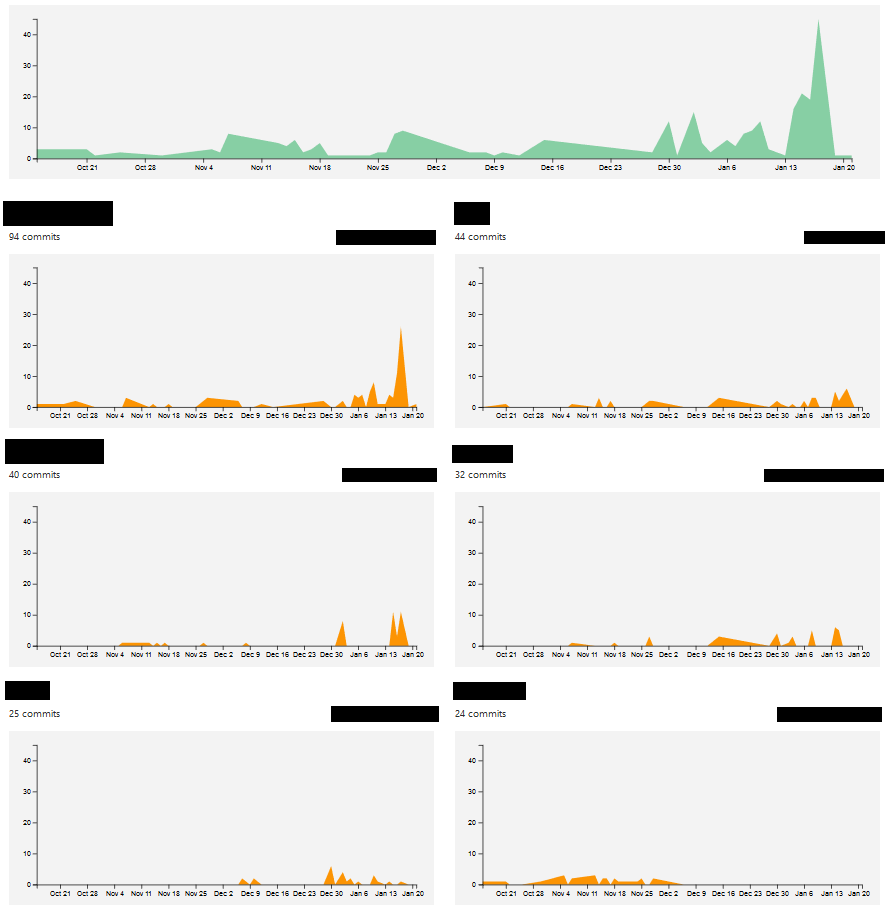
\includegraphics[scale=0.4]{slike/aktivnost.PNG} %veličina slike u odnosu na originalnu datoteku i pozicija slike
			\centering
			\caption{Primjer slike s potpisom}
			\label{fig:promjene}
		\end{figure}
		
		\begin{figure}[H]
			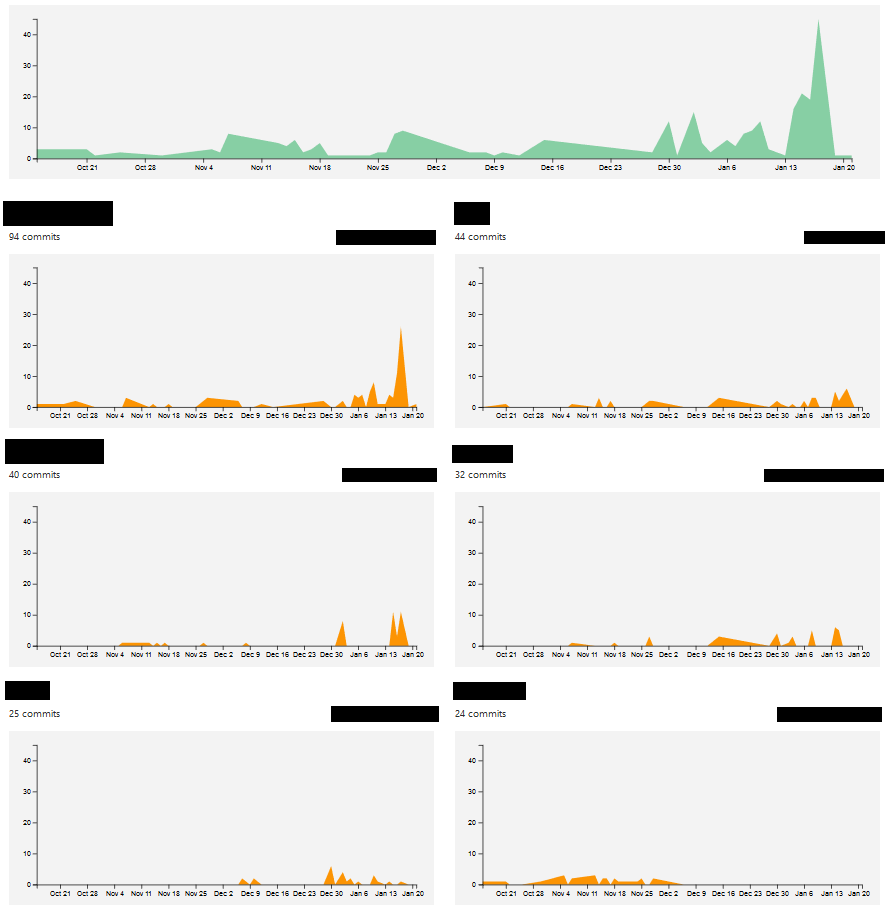
\includegraphics[width=\textwidth]{slike/aktivnost.PNG} %veličina u odnosu na širinu linije
			\caption{Primjer slike s potpisom 2}
			\label{fig:promjene2} %label mora biti drugaciji za svaku sliku
		\end{figure}
		
		Referenciranje slike \ref{fig:promjene2} u tekstu.
		
		\eject
		
	
	\chapter{Specifikacija programske potpore}
		
	\section{Funkcionalni zahtjevi}
			
			\noindent \textbf{Dionici:}
			
			\begin{packed_enum}
				\item Tragač na terenu
				\item Istraživač				
				\item Voditelj postaje
				\item Administrator
				
			\end{packed_enum}
			
			\noindent \textbf{Aktori i njihovi funkcionalni zahtjevi:}
			
			
			\begin{packed_enum}
				\item  \underbar{Neregistrirani korisnik  (inicijator) može:}
				
				\begin{packed_enum}
					\item se registrirati u sustav
					 \begin{packed_enum}
						\item  dati svoje podatke: korisničko ime, fotografija, lozinka, ime, prezime i email adresa
						\item  odabrati svoju ulogu(tragač, istraživač ili voditelj postaje)
						\item potvrditi registraciju na svojoj email adresi 
					\end{packed_enum}
				\end{packed_enum}
			
				\item  \underbar{Korisnik (inicijator) može:}
				
				\begin{packed_enum}
					\item se prijaviti u sustav
					\item upravljati svojim podatcima
					 \begin{packed_enum}
						\item  pregled osobnih podataka
						\item promjena osobnih podataka
						\item brisanje korisničkog računa
					\end{packed_enum}
				\end{packed_enum}

				\item  \underbar{Tragač na terenu (inicijator) može:}
				
				\begin{packed_enum}
					
					\item vidjeti zadatke tijekom akcije
					 \begin{packed_enum}
						\item označiti da je zadatak riješen
					\end{packed_enum}
					\item završiti akciju
					\item vidjeti gdje se nalaze ostali tragači na akciji 
					\item vidjeti koje su dostupne akcije 
					 \begin{packed_enum}
						\item prihvatiti akciju
						\item odbiti akciju
					\end{packed_enum} 
					\item vidjeti pozicije praćenih životinja
					\item odabrati vozilo kojim će ići u istraživanje
					\item vidjeti informacije o životinjama
					 \begin{packed_enum}
						\item dodati komentar
						\item izbrisati komentar
					\end{packed_enum}

					
				\end{packed_enum}

				\item  \underbar{Istraživač (inicijator) može:}
				
				\begin{packed_enum}

					\item vidjeti informacije o životinjama
					 \begin{packed_enum}
						\item dodati komentar
						\item izbrisati komentar
					\end{packed_enum}
					\item vidjeti kartu 
					 \begin{packed_enum}
						\item izraditi kartu: na temelju životinja ili tragača
					\end{packed_enum}
					\item stvoriti novu akciju
					 \begin{packed_enum}
						\item dodati nove zadatke
					\end{packed_enum}
					\item poslati voditelju postaje zahtjev za tragačima
					 \begin{packed_enum}
						\item dodati opis o željenim tragačima
					\end{packed_enum}
					\item zadati zadatke tragačima
					 \begin{packed_enum}
						\item upravljati zadacima
						 \begin{packed_enum}
							\item dodavati zadatke
							\item uređivati zadatke
							\item brisati zadatke
						\end{packed_enum}
						\item dodati komentare na zadatke
					\end{packed_enum}
					\item pregledati informacije


				\end{packed_enum}

				\item  \underbar{Voditelj postaje (inicijator) može:}
				
				\begin{packed_enum}
					\item pregledati sve tragače
					\item dodati tragača na akciju
					\item dodijeliti postaju tragaču
				\end{packed_enum}

				\item  \underbar{Administrator (inicijator) može:}
				
				\begin{packed_enum}
					\item vidjeti popis svih registriranih korisnika i njihovih osobnih podataka
					\item obrisati korisnika
					\item mijenjati dodijeljena prava i osobne podatke registriranim korisnicima
					\item potvrditi istraživača i voditelja postaje
				\end{packed_enum}

				\item  \underbar{Baza podataka (sudionik):}
				
				\begin{packed_enum}
					\item pohranjuje sve podatke o korisnicima 
					\item pohranjuje sve podatke o životinjama
					\item pohranjuje staze kojima tragači putuju(i način kojim su se kretali)
				\end{packed_enum}


			\end{packed_enum}
			
			\eject 
			
			
				
			\subsection{Obrasci uporabe}
								
				\subsubsection{Opis obrazaca uporabe}
					\textit{Funkcionalne zahtjeve razraditi u obliku obrazaca uporabe. Svaki obrazac je potrebno razraditi prema donjem predlošku. Ukoliko u nekom koraku može doći do odstupanja, potrebno je to odstupanje opisati i po mogućnosti ponuditi rješenje kojim bi se tijek obrasca vratio na osnovni tijek.}\\
					

					%%%%%%%%%%%%%%%%%%%%%%%%%%%%%%%%%%%%%%%%%%%%%%%%%%%%%%%%%%%%%%%%%%%%%%%%%%%%%%%%%%%%%%%%%%%%%%%%%%%%%%%%%%%%%%%%%%%%%%%%%%%%%%%%%%%%%%%%%%
					%%%%%%%%%%%%%%%%%%%%%%%%%%%%%%%%%%%%%%%%%%%%%%%%%%%%%          1         %%%%%%%%%%%%%%%%%%%%%%%%%%%%%%%%%%%%%%%%%%%%%%%%%%%%%%%%%%%%%%%%%
					%%%%%%%%%%%%%%%%%%%%%%%%%%%%%%%%%%%%%%%%%%%%%%%%%%%%%%%%%%%%%%%%%%%%%%%%%%%%%%%%%%%%%%%%%%%%%%%%%%%%%%%%%%%%%%%%%%%%%%%%%%%%%%%%%%%%%%%%%%
					\noindent \underbar{\textbf{UC1 - Registracija}}
					\begin{packed_item}
	
						\item \textbf{Glavni sudionik: }Neregistrirani korisnik
						\item  \textbf{Cilj:} Stvoriti korisnički račun 
						\item  \textbf{Sudionici:} Baza podataka
						\item  \textbf{Preduvjet:} -
						\item  \textbf{Opis osnovnog tijeka:} 
						
						
						\item[] \begin{packed_enum}
	
							\item Korisnik odabire opciju za registraciju							
							\item Korisnik unosi potrebne korisničke podatke
							\item Korisnik bira ulogu
							\item Ako je odabrana uloga voditelja postaje ili istraživača automatski se šalje zahtjev za potvrdu uloge administratoru i korisnik ne može nastaviti registraciju dok se ne potvrdi uloga
							\item Korisnik prima obavijest da registraciju mora potvrditi na mailu
							
						\end{packed_enum}
						
						\item  \textbf{Opis mogućih odstupanja:}
						
						\item[] \begin{packed_item}
	
							\item[2.a] Odabir već zauzetog korisničkog imena i/ili e-maila, unos korisničkog
							podatka u nedozvoljenom formatu ili pružanje neispravnoga e-maila
							
							\item[] \begin{packed_enum}
								
								\item Sustav obavještava korisnika o neuspjelom pokušaju i vraća ga na stranicu za registraciju 
								
							\end{packed_enum}
							%\item[2.b] $<$opis mogućeg scenarija odstupanja u koraku 2$>$
							%\item[4.a] $<$opis mogućeg scenarija odstupanja  u koraku 3$>$
							
						\end{packed_item}
					\end{packed_item}

					
					%%%%%%%%%%%%%%%%%%%%%%%%%%%%%%%%%%%%%%%%%%%%%%%%%%%%%%%%%%%%%%%%%%%%%%%%%%%%%%%%%%%%%%%%%%%%%%%%%%%%%%%%%%%%%%%%%%%%%%%%%%%%%%%%%%%%%%%%%%
					%%%%%%%%%%%%%%%%%%%%%%%%%%%%%%%%%%%%%%%%%%%%%%%%%%%%%          2         %%%%%%%%%%%%%%%%%%%%%%%%%%%%%%%%%%%%%%%%%%%%%%%%%%%%%%%%%%%%%%%%%
					%%%%%%%%%%%%%%%%%%%%%%%%%%%%%%%%%%%%%%%%%%%%%%%%%%%%%%%%%%%%%%%%%%%%%%%%%%%%%%%%%%%%%%%%%%%%%%%%%%%%%%%%%%%%%%%%%%%%%%%%%%%%%%%%%%%%%%%%%%

					\noindent \underbar{\textbf{UC2 - Potvrda preko maila}}
					\begin{packed_item}
	
						\item \textbf{Glavni sudionik: }Neregistrirani korisnik
						\item  \textbf{Cilj:} Potvrditi registraciju
						\item  \textbf{Sudionici:} Baza podataka
						\item  \textbf{Preduvjet:} Provedena prva dva koraka registracije
						\item  \textbf{Opis osnovnog tijeka:} 
						
						
						\item[] \begin{packed_enum}
	
							\item Korisnik dobiva mail sa poveznicom za potvrdu registracije						
							\item Korisnik klikne na link i preusmjerava se na početno sučelje aplikacije
							\item Ažurira se baza podataka
							
						\end{packed_enum}
						
						\item  \textbf{Opis mogućih odstupanja:}
						
						\item[] \begin{packed_item}
	
							\item[2.a] Neispravno korisničko ime/lozinka
							\item[] \begin{packed_enum}
								
								\item Sustav obavještava korisnika o neuspjelom pokušaju i vraća ga na stranicu za registraciju 
								
							\end{packed_enum}
							%\item[2.b] $<$opis mogućeg scenarija odstupanja u koraku 2$>$
							\item[3.a] Administrator odbija zahtjev za traženu ulogu
							\item[] \begin{packed_enum}
								
								\item Tog korisnika se preusmjerava natrag na biranje uloge bez mogućnosti odabira prijašnje
								
							\end{packed_enum}

						\end{packed_item}
					\end{packed_item}

					
					%%%%%%%%%%%%%%%%%%%%%%%%%%%%%%%%%%%%%%%%%%%%%%%%%%%%%%%%%%%%%%%%%%%%%%%%%%%%%%%%%%%%%%%%%%%%%%%%%%%%%%%%%%%%%%%%%%%%%%%%%%%%%%%%%%%%%%%%%%
					%%%%%%%%%%%%%%%%%%%%%%%%%%%%%%%%%%%%%%%%%%%%%%%%%%%%%          3         %%%%%%%%%%%%%%%%%%%%%%%%%%%%%%%%%%%%%%%%%%%%%%%%%%%%%%%%%%%%%%%%%
					%%%%%%%%%%%%%%%%%%%%%%%%%%%%%%%%%%%%%%%%%%%%%%%%%%%%%%%%%%%%%%%%%%%%%%%%%%%%%%%%%%%%%%%%%%%%%%%%%%%%%%%%%%%%%%%%%%%%%%%%%%%%%%%%%%%%%%%%%%


					\noindent \underbar{\textbf{UC3 - Prijava u sustav}}
					\begin{packed_item}
	
						\item \textbf{Glavni sudionik: }Korisnik (voditelj postaje, tragač, istraživač)
						\item  \textbf{Cilj:} Pristup registriranog korisnika korisničkom sučelju
						\item  \textbf{Sudionici:} Baza podataka
						\item  \textbf{Preduvjet:} Registracija
						\item  \textbf{Opis osnovnog tijeka:} 
						
						
						\item[] \begin{packed_enum}
	
							\item Unos korisničkog imena i lozinke							
							\item Potvrda o ispravnosti unesenih podataka
							\item Pristup korisničkim funkcijama
							
						\end{packed_enum}
						
						\item  \textbf{Opis mogućih odstupanja:}
						
						\item[] \begin{packed_item}
	
							\item[2.a] Neispravno korisničko ime/lozinka
							\item[] \begin{packed_enum}
								
								\item Sustav obavještava korisnika o neuspjelom pokušaju i vraća ga na stranicu za registraciju 
								
							\end{packed_enum}
							%\item[2.b] $<$opis mogućeg scenarija odstupanja u koraku 2$>$
							%\item[3.a] $<$opis mogućeg scenarija odstupanja  u koraku 3$>$
							
						\end{packed_item}
					\end{packed_item}
					
					%%%%%%%%%%%%%%%%%%%%%%%%%%%%%%%%%%%%%%%%%%%%%%%%%%%%%%%%%%%%%%%%%%%%%%%%%%%%%%%%%%%%%%%%%%%%%%%%%%%%%%%%%%%%%%%%%%%%%%%%%%%%%%%%%%%%%%%%%%
					%%%%%%%%%%%%%%%%%%%%%%%%%%%%%%%%%%%%%%%%%%%%%%%%%%%%%          4         %%%%%%%%%%%%%%%%%%%%%%%%%%%%%%%%%%%%%%%%%%%%%%%%%%%%%%%%%%%%%%%%%
					%%%%%%%%%%%%%%%%%%%%%%%%%%%%%%%%%%%%%%%%%%%%%%%%%%%%%%%%%%%%%%%%%%%%%%%%%%%%%%%%%%%%%%%%%%%%%%%%%%%%%%%%%%%%%%%%%%%%%%%%%%%%%%%%%%%%%%%%%%

					\noindent \underbar{\textbf{UC4 - Odjava iz sustava}}
					\begin{packed_item}
	
						\item \textbf{Glavni sudionik: }  Korisnik (voditelj postaje, tragač, istraživač)
						\item  \textbf{Cilj:} Odjava prijavljenog korisnika iz sustava
						\item  \textbf{Sudionici:} Baza podataka
						\item  \textbf{Preduvjet:} Korisnik je prijavljen
						\item  \textbf{Opis osnovnog tijeka:} 
						
						
						\item[] \begin{packed_enum}
	
							\item Korisnik odabire opciju odjava							
							\item Korisnik je vraćen na stranicu za prijavu
						
						\end{packed_enum}
				
							
					\end{packed_item}

					%%%%%%%%%%%%%%%%%%%%%%%%%%%%%%%%%%%%%%%%%%%%%%%%%%%%%%%%%%%%%%%%%%%%%%%%%%%%%%%%%%%%%%%%%%%%%%%%%%%%%%%%%%%%%%%%%%%%%%%%%%%%%%%%%%%%%%%%%%
					%%%%%%%%%%%%%%%%%%%%%%%%%%%%%%%%%%%%%%%%%%%%%%%%%%%%%          5         %%%%%%%%%%%%%%%%%%%%%%%%%%%%%%%%%%%%%%%%%%%%%%%%%%%%%%%%%%%%%%%%%
					%%%%%%%%%%%%%%%%%%%%%%%%%%%%%%%%%%%%%%%%%%%%%%%%%%%%%%%%%%%%%%%%%%%%%%%%%%%%%%%%%%%%%%%%%%%%%%%%%%%%%%%%%%%%%%%%%%%%%%%%%%%%%%%%%%%%%%%%%%

					\noindent \underbar{\textbf{UC5 - Pregled svojih osobnih podataka}}
					\begin{packed_item}
	
						\item \textbf{Glavni sudionik: }  Korisnik
						\item  \textbf{Cilj:} Pregled svojih osobnih podataka
						\item  \textbf{Sudionici:} Baza podataka
						\item  \textbf{Preduvjet:} -
						\item  \textbf{Opis osnovnog tijeka:} 
						
						
						\item[] \begin{packed_enum}
	
							\item Korisnik bira opciju ”pregled svojih osobnih podataka”				
							\item Korisnik vidi svoje osobne podatke
							
						\end{packed_enum}
					\end{packed_item}

					%%%%%%%%%%%%%%%%%%%%%%%%%%%%%%%%%%%%%%%%%%%%%%%%%%%%%%%%%%%%%%%%%%%%%%%%%%%%%%%%%%%%%%%%%%%%%%%%%%%%%%%%%%%%%%%%%%%%%%%%%%%%%%%%%%%%%%%%%%
					%%%%%%%%%%%%%%%%%%%%%%%%%%%%%%%%%%%%%%%%%%%%%%%%%%%%%          6         %%%%%%%%%%%%%%%%%%%%%%%%%%%%%%%%%%%%%%%%%%%%%%%%%%%%%%%%%%%%%%%%%
					%%%%%%%%%%%%%%%%%%%%%%%%%%%%%%%%%%%%%%%%%%%%%%%%%%%%%%%%%%%%%%%%%%%%%%%%%%%%%%%%%%%%%%%%%%%%%%%%%%%%%%%%%%%%%%%%%%%%%%%%%%%%%%%%%%%%%%%%%%
					\noindent \underbar{\textbf{UC6 - Pregled korisnika}}
					\begin{packed_item}
	
						\item \textbf{Glavni sudionik: }  Administrator
						\item  \textbf{Cilj:} Pregledati registrirane korisnike
						\item  \textbf{Sudionici:} Baza podataka
						\item  \textbf{Preduvjet:} Korisnik je registriran i dodijeljena su mu prava administratora
						\item  \textbf{Opis osnovnog tijeka:} 
						
						
						\item[] \begin{packed_enum}
	
							\item Administrator odabire opciju pregledavanja korisnika 						
							\item Prikaz liste svih ispravno registriranih korisnika i njihovih osobnih podataka
							
						\end{packed_enum}
					\end{packed_item}
					%%%%%%%%%%%%%%%%%%%%%%%%%%%%%%%%%%%%%%%%%%%%%%%%%%%%%%%%%%%%%%%%%%%%%%%%%%%%%%%%%%%%%%%%%%%%%%%%%%%%%%%%%%%%%%%%%%%%%%%%%%%%%%%%%%%%%%%%%%
					%%%%%%%%%%%%%%%%%%%%%%%%%%%%%%%%%%%%%%%%%%%%%%%%%%%%%          7         %%%%%%%%%%%%%%%%%%%%%%%%%%%%%%%%%%%%%%%%%%%%%%%%%%%%%%%%%%%%%%%%%
					%%%%%%%%%%%%%%%%%%%%%%%%%%%%%%%%%%%%%%%%%%%%%%%%%%%%%%%%%%%%%%%%%%%%%%%%%%%%%%%%%%%%%%%%%%%%%%%%%%%%%%%%%%%%%%%%%%%%%%%%%%%%%%%%%%%%%%%%%%
					\noindent \underbar{\textbf{UC7 - Brisanje korisnika}}
					\begin{packed_item}
	
						\item \textbf{Glavni sudionik: }  Administrator
						\item  \textbf{Cilj:} Obrisati korisnički račun
						\item  \textbf{Sudionici:} Baza podataka
						\item  \textbf{Preduvjet:} Postoji korisnički račun
						\item  \textbf{Opis osnovnog tijeka:} 
						
						
						\item[] \begin{packed_enum}
	
							\item  Administrator odabire opciju “pregled korisnika”	
							\item Administrator odabire jedan ili više korisničkih računa
							\item Administrator odabire opciju za brisanje odabranih računa
							\item Baza podataka se ažurira	
							
						\end{packed_enum}
					\end{packed_item}
					%%%%%%%%%%%%%%%%%%%%%%%%%%%%%%%%%%%%%%%%%%%%%%%%%%%%%%%%%%%%%%%%%%%%%%%%%%%%%%%%%%%%%%%%%%%%%%%%%%%%%%%%%%%%%%%%%%%%%%%%%%%%%%%%%%%%%%%%%%
					%%%%%%%%%%%%%%%%%%%%%%%%%%%%%%%%%%%%%%%%%%%%%%%%%%%%%          8         %%%%%%%%%%%%%%%%%%%%%%%%%%%%%%%%%%%%%%%%%%%%%%%%%%%%%%%%%%%%%%%%%
					%%%%%%%%%%%%%%%%%%%%%%%%%%%%%%%%%%%%%%%%%%%%%%%%%%%%%%%%%%%%%%%%%%%%%%%%%%%%%%%%%%%%%%%%%%%%%%%%%%%%%%%%%%%%%%%%%%%%%%%%%%%%%%%%%%%%%%%%%%
					\noindent \underbar{\textbf{UC8 Pregled osobnih podataka}}
					\begin{packed_item}
	
						\item \textbf{Glavni sudionik: }  Administrator
						\item  \textbf{Cilj:} Pregled osobnih podataka
						\item  \textbf{Sudionici:} Baza podataka
						\item  \textbf{Preduvjet:} Postoji barem jedan korisniči račun
						\item  \textbf{Opis osnovnog tijeka:} 
						
						
						\item[] \begin{packed_enum}
	
							\item Administrator odabire opciju “pregled korisnika”													
							\item Administrator odabire korisnički račun
							\item Administrator odabire opciju “pregled osobnih podataka”
							\item Prikazuju se osobni podatci
							
						\end{packed_enum}
					\end{packed_item}
					%%%%%%%%%%%%%%%%%%%%%%%%%%%%%%%%%%%%%%%%%%%%%%%%%%%%%%%%%%%%%%%%%%%%%%%%%%%%%%%%%%%%%%%%%%%%%%%%%%%%%%%%%%%%%%%%%%%%%%%%%%%%%%%%%%%%%%%%%%
					%%%%%%%%%%%%%%%%%%%%%%%%%%%%%%%%%%%%%%%%%%%%%%%%%%%%%          9         %%%%%%%%%%%%%%%%%%%%%%%%%%%%%%%%%%%%%%%%%%%%%%%%%%%%%%%%%%%%%%%%%
					%%%%%%%%%%%%%%%%%%%%%%%%%%%%%%%%%%%%%%%%%%%%%%%%%%%%%%%%%%%%%%%%%%%%%%%%%%%%%%%%%%%%%%%%%%%%%%%%%%%%%%%%%%%%%%%%%%%%%%%%%%%%%%%%%%%%%%%%%%
					\noindent \underbar{\textbf{UC9 - Promjena dodjeljenih prava}}
					\begin{packed_item}
	
						\item \textbf{Glavni sudionik: }  Administrator
						\item  \textbf{Cilj:} Promijeniti prava korisnika
						\item  \textbf{Sudionici:} Baza podataka
						\item  \textbf{Preduvjet:} Postoji barem jedan korisniči račun
						\item  \textbf{Opis osnovnog tijeka:} 
						
						
						\item[] \begin{packed_enum}
	
							\item Administrator odabire opciju “pregled korisnika”
							\item Administrator odabire pregled osobnih podataka određenog korisnika
							\item Administrator odabire opciju za promjenu dodjeljenih prava korisnika
							\item Administrator označava prava koja korisnik treba imat
							\item Administrator sprema promjene
							\item Baza podataka se ažurira
							
						\end{packed_enum}
						
						\item  \textbf{Opis mogućih odstupanja:}
						
						\item[] \begin{packed_item}
	
							\item[1.a] Administrator nakon promjene prava ne odabere opciju 
							„Spremi“
							
							
							\item[] \begin{packed_enum}
								
								\item Sustav obavještava administratora da nije spremio prava 
								prije izlaska iz prozora 
								
							\end{packed_enum}
							%\item[2.b] $<$opis mogućeg scenarija odstupanja u koraku 2$>$
							%\item[4.a] $<$opis mogućeg scenarija odstupanja  u koraku 3$>$
							
						\end{packed_item}
					\end{packed_item}
					%%%%%%%%%%%%%%%%%%%%%%%%%%%%%%%%%%%%%%%%%%%%%%%%%%%%%%%%%%%%%%%%%%%%%%%%%%%%%%%%%%%%%%%%%%%%%%%%%%%%%%%%%%%%%%%%%%%%%%%%%%%%%%%%%%%%%%%%%%
					%%%%%%%%%%%%%%%%%%%%%%%%%%%%%%%%%%%%%%%%%%%%%%%%%%%%%          10         %%%%%%%%%%%%%%%%%%%%%%%%%%%%%%%%%%%%%%%%%%%%%%%%%%%%%%%%%%%%%%%%
					%%%%%%%%%%%%%%%%%%%%%%%%%%%%%%%%%%%%%%%%%%%%%%%%%%%%%%%%%%%%%%%%%%%%%%%%%%%%%%%%%%%%%%%%%%%%%%%%%%%%%%%%%%%%%%%%%%%%%%%%%%%%%%%%%%%%%%%%%%
					\noindent \underbar{\textbf{UC10 - Promjena osobnih podataka}}
					\begin{packed_item}
	
						\item \textbf{Glavni sudionik: }  Administrator
						\item  \textbf{Cilj:} Promjena osobnih podataka korisnika
						\item  \textbf{Sudionici:} Baza podataka
						\item  \textbf{Preduvjet:} Postoji barem jedan korisnički račun
						\item  \textbf{Opis osnovnog tijeka:} 
						
						
						\item[] \begin{packed_enum}
	
							\item Administrator odabire opciji za promjenu podataka				
							\item Administrator mijenja osobne podatke
							\item Administrator sprema promjene
							\item Baza podataka se ažurira
							
						\end{packed_enum}
						
						\item  \textbf{Opis mogućih odstupanja:}
						
						\item[] \begin{packed_item}
	
							\item[1.a] Administrator nakon promjene podataka ne odabere opciju 
							„Spremi“
							
							
							\item[] \begin{packed_enum}
								
								\item Sustav obavještava administratora da nije spremio podatke 
								prije izlaska iz prozora
								
							\end{packed_enum}
							
						\end{packed_item}
					\end{packed_item}
					%%%%%%%%%%%%%%%%%%%%%%%%%%%%%%%%%%%%%%%%%%%%%%%%%%%%%%%%%%%%%%%%%%%%%%%%%%%%%%%%%%%%%%%%%%%%%%%%%%%%%%%%%%%%%%%%%%%%%%%%%%%%%%%%%%%%%%%%%%
					%%%%%%%%%%%%%%%%%%%%%%%%%%%%%%%%%%%%%%%%%%%%%%%%%%%%%          11         %%%%%%%%%%%%%%%%%%%%%%%%%%%%%%%%%%%%%%%%%%%%%%%%%%%%%%%%%%%%%%%%
					%%%%%%%%%%%%%%%%%%%%%%%%%%%%%%%%%%%%%%%%%%%%%%%%%%%%%%%%%%%%%%%%%%%%%%%%%%%%%%%%%%%%%%%%%%%%%%%%%%%%%%%%%%%%%%%%%%%%%%%%%%%%%%%%%%%%%%%%%%
					\noindent \underbar{\textbf{UC11 - Potvrda istraživača i voditelja postaje}}
					\begin{packed_item}
	
						\item \textbf{Glavni sudionik: }  Administrator
						\item  \textbf{Cilj:} Potvrđuje ili odbija zahtjeve za određene ulog
						\item  \textbf{Sudionici:} Baza podataka
						\item  \textbf{Preduvjet:} Postoje zahtjevi za odabrane uloge
						\item  \textbf{Opis osnovnog tijeka:} 
						
						
						\item[] \begin{packed_enum}
	
							\item Administratoru dolazi zahtjev
							\item Bira opcije „Potvrdi“ ili „Odbij“
							\item Baza podataka se ažurira
							\item Odgovor administartora šalje se osobi koja je poslala zahtjev
							
						\end{packed_enum}
					\end{packed_item}
					%%%%%%%%%%%%%%%%%%%%%%%%%%%%%%%%%%%%%%%%%%%%%%%%%%%%%%%%%%%%%%%%%%%%%%%%%%%%%%%%%%%%%%%%%%%%%%%%%%%%%%%%%%%%%%%%%%%%%%%%%%%%%%%%%%%%%%%%%%
					%%%%%%%%%%%%%%%%%%%%%%%%%%%%%%%%%%%%%%%%%%%%%%%%%%%%%          12         %%%%%%%%%%%%%%%%%%%%%%%%%%%%%%%%%%%%%%%%%%%%%%%%%%%%%%%%%%%%%%%%%
					%%%%%%%%%%%%%%%%%%%%%%%%%%%%%%%%%%%%%%%%%%%%%%%%%%%%%%%%%%%%%%%%%%%%%%%%%%%%%%%%%%%%%%%%%%%%%%%%%%%%%%%%%%%%%%%%%%%%%%%%%%%%%%%%%%%%%%%%%%
					\noindent \underbar{\textbf{UC12 - Pregled svojih tragača}}
					\begin{packed_item}
	
						\item \textbf{Glavni sudionik: }  Voditelj postaje
						\item  \textbf{Cilj:} Pregled vlastite postaje
						\item  \textbf{Sudionici:} Baza podataka
						\item  \textbf{Preduvjet:} Voditelj je već odabrao barem jednog tragača
						\item  \textbf{Opis osnovnog tijeka:} 
						
						
						\item[] \begin{packed_enum}
	
							\item Voditelj postaje odabire opciju pregled svojih tragača		
							\item Pojavljuje se lista njih
							
						\end{packed_enum}
					\end{packed_item}
					%%%%%%%%%%%%%%%%%%%%%%%%%%%%%%%%%%%%%%%%%%%%%%%%%%%%%%%%%%%%%%%%%%%%%%%%%%%%%%%%%%%%%%%%%%%%%%%%%%%%%%%%%%%%%%%%%%%%%%%%%%%%%%%%%%%%%%%%%%
					%%%%%%%%%%%%%%%%%%%%%%%%%%%%%%%%%%%%%%%%%%%%%%%%%%%%%          13         %%%%%%%%%%%%%%%%%%%%%%%%%%%%%%%%%%%%%%%%%%%%%%%%%%%%%%%%%%%%%%%%
					%%%%%%%%%%%%%%%%%%%%%%%%%%%%%%%%%%%%%%%%%%%%%%%%%%%%%%%%%%%%%%%%%%%%%%%%%%%%%%%%%%%%%%%%%%%%%%%%%%%%%%%%%%%%%%%%%%%%%%%%%%%%%%%%%%%%%%%%%%
					\noindent \underbar{\textbf{UC13 - Uređivanje sposobnosti tragača}}
					\begin{packed_item}
	
						\item \textbf{Glavni sudionik: }  Voditelj postaje
						\item  \textbf{Cilj:} Uređivanje sposobnosti tragača
						\item  \textbf{Sudionici:} Baza podataka
						\item  \textbf{Preduvjet:} Voditelj je odabrao barem jednpog tragača
						\item  \textbf{Opis osnovnog tijeka:} 
						
						
						\item[] \begin{packed_enum}
	
							\item Voditelj postaje odabire opciju pregled svojih tragača
							\item Pojavljuje se lista njih
							\item Voditelj bira tragača
							\item Voditelj bira opciju uređivanje sposobnosti tragača
							\item Voditelj označuje sposobnosti za koje je tragač sposoban
							\item Baza podataka se ažurira	
							
						\end{packed_enum}
					\end{packed_item}
					%%%%%%%%%%%%%%%%%%%%%%%%%%%%%%%%%%%%%%%%%%%%%%%%%%%%%%%%%%%%%%%%%%%%%%%%%%%%%%%%%%%%%%%%%%%%%%%%%%%%%%%%%%%%%%%%%%%%%%%%%%%%%%%%%%%%%%%%%%
					%%%%%%%%%%%%%%%%%%%%%%%%%%%%%%%%%%%%%%%%%%%%%%%%%%%%%          14         %%%%%%%%%%%%%%%%%%%%%%%%%%%%%%%%%%%%%%%%%%%%%%%%%%%%%%%%%%%%%%%%
					%%%%%%%%%%%%%%%%%%%%%%%%%%%%%%%%%%%%%%%%%%%%%%%%%%%%%%%%%%%%%%%%%%%%%%%%%%%%%%%%%%%%%%%%%%%%%%%%%%%%%%%%%%%%%%%%%%%%%%%%%%%%%%%%%%%%%%%%%%
					\noindent \underbar{\textbf{UC14 - Pregled svih tragača}}
					\begin{packed_item}
	
						\item \textbf{Glavni sudionik: }  Voditelj postaje
						\item  \textbf{Cilj:} Pregledati nesvrstane tragače
						\item  \textbf{Sudionici:} Baza podataka
						\item  \textbf{Preduvjet:} Postoje nesvrstani tragači
						\item  \textbf{Opis osnovnog tijeka:} 
						
						
						\item[] \begin{packed_enum}
	
							\item Voditelj postaje odabire opciju pregled nesvrstanih tragača						
							\item Pojavljuje se lista njih
							
						\end{packed_enum}
					\end{packed_item}
					%%%%%%%%%%%%%%%%%%%%%%%%%%%%%%%%%%%%%%%%%%%%%%%%%%%%%%%%%%%%%%%%%%%%%%%%%%%%%%%%%%%%%%%%%%%%%%%%%%%%%%%%%%%%%%%%%%%%%%%%%%%%%%%%%%%%%%%%%%
					%%%%%%%%%%%%%%%%%%%%%%%%%%%%%%%%%%%%%%%%%%%%%%%%%%%%%          15         %%%%%%%%%%%%%%%%%%%%%%%%%%%%%%%%%%%%%%%%%%%%%%%%%%%%%%%%%%%%%%%%
					%%%%%%%%%%%%%%%%%%%%%%%%%%%%%%%%%%%%%%%%%%%%%%%%%%%%%%%%%%%%%%%%%%%%%%%%%%%%%%%%%%%%%%%%%%%%%%%%%%%%%%%%%%%%%%%%%%%%%%%%%%%%%%%%%%%%%%%%%%
					\noindent \underbar{\textbf{UC15 - Odabir tragača za postaju}}
					\begin{packed_item}
	
						\item \textbf{Glavni sudionik: }  Voditelj postaje
						\item  \textbf{Cilj:} iz nesvrstanih tragača voditelj postaje bira one za svoju postaju
						\item  \textbf{Sudionici:} Baza podataka
						\item  \textbf{Preduvjet:} Korisnik je u ulozi voditelja i postoje nesvrstani tragači
						\item  \textbf{Opis osnovnog tijeka:} 
						
						
						\item[] \begin{packed_enum}
	
							\item Voditelj bira opciju dodavanja postaje tragaču
							\item  Voditelj pregledava nesvrstane tragače
							\item  Voditelj odabire jednog ili više tragača za svoju postaju
							\item  Voditelj dodjeljuje spodobnosti odabranima
							\item Odabranim tragačima dolazi obavijest za kou su postaju odabran
							
						\end{packed_enum}
					\end{packed_item}
					%%%%%%%%%%%%%%%%%%%%%%%%%%%%%%%%%%%%%%%%%%%%%%%%%%%%%%%%%%%%%%%%%%%%%%%%%%%%%%%%%%%%%%%%%%%%%%%%%%%%%%%%%%%%%%%%%%%%%%%%%%%%%%%%%%%%%%%%%%
					%%%%%%%%%%%%%%%%%%%%%%%%%%%%%%%%%%%%%%%%%%%%%%%%%%%%%          16         %%%%%%%%%%%%%%%%%%%%%%%%%%%%%%%%%%%%%%%%%%%%%%%%%%%%%%%%%%%%%%%%
					%%%%%%%%%%%%%%%%%%%%%%%%%%%%%%%%%%%%%%%%%%%%%%%%%%%%%%%%%%%%%%%%%%%%%%%%%%%%%%%%%%%%%%%%%%%%%%%%%%%%%%%%%%%%%%%%%%%%%%%%%%%%%%%%%%%%%%%%%%
					\noindent \underbar{\textbf{UC16 - Određivanje sposobnosti tragača}}
					\begin{packed_item}
	
						\item \textbf{Glavni sudionik: }  Voditelj postaje
						\item  \textbf{Cilj:} Određivanje sposobnosti tragača
						\item  \textbf{Sudionici:} Baza podataka
						\item  \textbf{Preduvjet:} Voditelj je odabrao barem jednog tragača
						\item  \textbf{Opis osnovnog tijeka:} 
						
						
						\item[] \begin{packed_enum}
	
							\item Pojavljuje se lista upravo odabranih tragača
							\item Voditelj dodaje sposobnosti svakom od njih
							\item Voditelj potvrđuje promjene
							\item Ažurira se baza podataka	

						\end{packed_enum}
					\end{packed_item}
					%%%%%%%%%%%%%%%%%%%%%%%%%%%%%%%%%%%%%%%%%%%%%%%%%%%%%%%%%%%%%%%%%%%%%%%%%%%%%%%%%%%%%%%%%%%%%%%%%%%%%%%%%%%%%%%%%%%%%%%%%%%%%%%%%%%%%%%%%%
					%%%%%%%%%%%%%%%%%%%%%%%%%%%%%%%%%%%%%%%%%%%%%%%%%%%%%          17         %%%%%%%%%%%%%%%%%%%%%%%%%%%%%%%%%%%%%%%%%%%%%%%%%%%%%%%%%%%%%%%%
					%%%%%%%%%%%%%%%%%%%%%%%%%%%%%%%%%%%%%%%%%%%%%%%%%%%%%%%%%%%%%%%%%%%%%%%%%%%%%%%%%%%%%%%%%%%%%%%%%%%%%%%%%%%%%%%%%%%%%%%%%%%%%%%%%%%%%%%%%%
					\noindent \underbar{\textbf{UC17 - Pregled akcija}}
					\begin{packed_item}
	
						\item \textbf{Glavni sudionik: } Voditelj postaje
						\item  \textbf{Cilj:} Pregled akcija u tijeku
						\item  \textbf{Sudionici:} Baza podataka
						\item  \textbf{Preduvjet:} Postoji akcija u tijeku
						\item  \textbf{Opis osnovnog tijeka:} 
						
						
						\item[] \begin{packed_enum}
	
							\item Voditelj postaje bira opciju “pregled akcija”
							\item Pojavljuje se lista aktivnih akcija
							
						\end{packed_enum}
					\end{packed_item}
					%%%%%%%%%%%%%%%%%%%%%%%%%%%%%%%%%%%%%%%%%%%%%%%%%%%%%%%%%%%%%%%%%%%%%%%%%%%%%%%%%%%%%%%%%%%%%%%%%%%%%%%%%%%%%%%%%%%%%%%%%%%%%%%%%%%%%%%%%%
					%%%%%%%%%%%%%%%%%%%%%%%%%%%%%%%%%%%%%%%%%%%%%%%%%%%%%          18         %%%%%%%%%%%%%%%%%%%%%%%%%%%%%%%%%%%%%%%%%%%%%%%%%%%%%%%%%%%%%%%%
					%%%%%%%%%%%%%%%%%%%%%%%%%%%%%%%%%%%%%%%%%%%%%%%%%%%%%%%%%%%%%%%%%%%%%%%%%%%%%%%%%%%%%%%%%%%%%%%%%%%%%%%%%%%%%%%%%%%%%%%%%%%%%%%%%%%%%%%%%%
					\noindent \underbar{\textbf{UC18 - Pregled zahtjeva}}
					\begin{packed_item}
	
						\item \textbf{Glavni sudionik: }  Voditelj postaje
						\item  \textbf{Cilj:} Pregled zahtjeva
						\item  \textbf{Sudionici:} Baza podataka
						\item  \textbf{Preduvjet:} Postoji neizvršeni zahtjev
						\item  \textbf{Opis osnovnog tijeka:} 
						
						
						\item[] \begin{packed_enum}
	
							\item Voditelj postaje bira opciju “pregled zahtjeva”
							\item Pojavljuje se lista neizvršenih zahtjeva
							
						\end{packed_enum}
					\end{packed_item}
					%%%%%%%%%%%%%%%%%%%%%%%%%%%%%%%%%%%%%%%%%%%%%%%%%%%%%%%%%%%%%%%%%%%%%%%%%%%%%%%%%%%%%%%%%%%%%%%%%%%%%%%%%%%%%%%%%%%%%%%%%%%%%%%%%%%%%%%%%%
					%%%%%%%%%%%%%%%%%%%%%%%%%%%%%%%%%%%%%%%%%%%%%%%%%%%%%          19         %%%%%%%%%%%%%%%%%%%%%%%%%%%%%%%%%%%%%%%%%%%%%%%%%%%%%%%%%%%%%%%%
					%%%%%%%%%%%%%%%%%%%%%%%%%%%%%%%%%%%%%%%%%%%%%%%%%%%%%%%%%%%%%%%%%%%%%%%%%%%%%%%%%%%%%%%%%%%%%%%%%%%%%%%%%%%%%%%%%%%%%%%%%%%%%%%%%%%%%%%%%%
					\noindent \underbar{\textbf{UC19 - Dodavanje tragača na akciju}}
					\begin{packed_item}
	
						\item \textbf{Glavni sudionik: }  Voditelj postaje
						\item  \textbf{Cilj:} Dodati tragača na akciju
						\item  \textbf{Sudionici:} Baza podataka
						\item  \textbf{Preduvjet:}  Postoji zahtjev za tragačima
						\item  \textbf{Opis osnovnog tijeka:} 
						
						
						\item[] \begin{packed_enum}
	
							\item Voditelj postaje odabire opciju pregled zahtjeva ili opciju pregled akcija 
							\item Voditelj postaje bira zahtjev ili akciju	
							\item Voditelj postaje izabire opciju “pregled svojih tragača” (u oba slučaja)
							\item Voditelj postaje izabire tragača I odabire opciju “dodaj u akciju”
							\item Zahtjev se može označiti kao izvršen 
							\item Baza podataka se ažurira
						\end{packed_enum}
					\end{packed_item}

					%%%%%%%%%%%%%%%%%%%%%%%%%%%%%%%%%%%%%%%%%%%%%%%%%%%%%%%%%%%%%%%%%%%%%%%%%%%%%%%%%%%%%%%%%%%%%%%%%%%%%%%%%%%%%%%%%%%%%%%%%%%%%%%%%%%%%%%%%%
					%%%%%%%%%%%%%%%%%%%%%%%%%%%%%%%%%%%%%%%%%%%%%%%%%%%%%          20         %%%%%%%%%%%%%%%%%%%%%%%%%%%%%%%%%%%%%%%%%%%%%%%%%%%%%%%%%%%%%%%%
					%%%%%%%%%%%%%%%%%%%%%%%%%%%%%%%%%%%%%%%%%%%%%%%%%%%%%%%%%%%%%%%%%%%%%%%%%%%%%%%%%%%%%%%%%%%%%%%%%%%%%%%%%%%%%%%%%%%%%%%%%%%%%%%%%%%%%%%%%%

					\noindent \underbar{\textbf{UC20 - Pregled informacija o životinjama}}
					\begin{packed_item}
	
						\item \textbf{Glavni sudionik: } Istraživač, tragač
						\item  \textbf{Cilj:} Pregledati informacije o životinji
						\item  \textbf{Sudionici:} Baza podataka
						\item  \textbf{Preduvjet:} -
						\item  \textbf{Opis osnovnog tijeka:}
						
						\item[] \begin{packed_enum}
	
							\item Glavni sudionik odabire životinju na karti
							\item	Prikazuju se informacije o životinji
						
						\end{packed_enum}
					\end{packed_item}
				
					%%%%%%%%%%%%%%%%%%%%%%%%%%%%%%%%%%%%%%%%%%%%%%%%%%%%%%%%%%%%%%%%%%%%%%%%%%%%%%%%%%%%%%%%%%%%%%%%%%%%%%%%%%%%%%%%%%%%%%%%%%%%%%%%%%%%%%%%%%
					%%%%%%%%%%%%%%%%%%%%%%%%%%%%%%%%%%%%%%%%%%%%%%%%%%%%%          21         %%%%%%%%%%%%%%%%%%%%%%%%%%%%%%%%%%%%%%%%%%%%%%%%%%%%%%%%%%%%%%%%
					%%%%%%%%%%%%%%%%%%%%%%%%%%%%%%%%%%%%%%%%%%%%%%%%%%%%%%%%%%%%%%%%%%%%%%%%%%%%%%%%%%%%%%%%%%%%%%%%%%%%%%%%%%%%%%%%%%%%%%%%%%%%%%%%%%%%%%%%%%
					\noindent \underbar{\textbf{UC21 - Dodavanje komentara o životinjama }}
					\begin{packed_item}
	
						\item \textbf{Glavni sudionik: }: Tragač ili iistraživač 
						\item  \textbf{Cilj:} Dodavanje komentara o praćenoj životinji
						\item  \textbf{Sudionici:} Baza podataka
						\item  \textbf{Preduvjet:}Korisnik je u ulozi tragača i pratio je životinju o kojoj piše komentar ili je istraživač koji je započeo akciju
						\item  \textbf{Opis osnovnog tijeka:}
						
						\item[] \begin{packed_enum}
	
							\item Tragač ili istraživač odabire životinju o kojoj želi napisati komentar
							\item Tragač ili istraživač odabire opciju pisanja komentara
							\item   Tragač ili istraživač piše komentar
							\item  Tragač ili istraživač potvrđuje komentar
							\item  Ažurira se baza podataka
							
						\end{packed_enum}
					\end{packed_item}
					%%%%%%%%%%%%%%%%%%%%%%%%%%%%%%%%%%%%%%%%%%%%%%%%%%%%%%%%%%%%%%%%%%%%%%%%%%%%%%%%%%%%%%%%%%%%%%%%%%%%%%%%%%%%%%%%%%%%%%%%%%%%%%%%%%%%%%%%%%
					%%%%%%%%%%%%%%%%%%%%%%%%%%%%%%%%%%%%%%%%%%%%%%%%%%%%%          22         %%%%%%%%%%%%%%%%%%%%%%%%%%%%%%%%%%%%%%%%%%%%%%%%%%%%%%%%%%%%%%%%
					%%%%%%%%%%%%%%%%%%%%%%%%%%%%%%%%%%%%%%%%%%%%%%%%%%%%%%%%%%%%%%%%%%%%%%%%%%%%%%%%%%%%%%%%%%%%%%%%%%%%%%%%%%%%%%%%%%%%%%%%%%%%%%%%%%%%%%%%%%
					\noindent \underbar{\textbf{UC22 - Brisanje komentara}}
					\begin{packed_item}
	
						\item \textbf{Glavni sudionik: }Tragač ili iistraživač 
						\item  \textbf{Cilj:} brisanje komentara o životinji
						\item  \textbf{Sudionici:} Baza podataka
						\item  \textbf{Preduvjet:} Korisnik je u ulozi tragača i pratio je životinju o kojoj piše komentar ili je istraživač koji je započeo akciju
						\item  \textbf{Opis osnovnog tijeka:}
						
						\item[] \begin{packed_enum}
	
							\item Tragač ili istraživač odabire životinju o kojoj želi izbrisati komentar
							\item Tragač ili istraživač odabire komentar koji želi izbrisati
							\item Tragač ili istraživač odabire opciju brisanja komentara
							\item Ažurira se baza podataka
							
						\end{packed_enum}
					\end{packed_item}
					%%%%%%%%%%%%%%%%%%%%%%%%%%%%%%%%%%%%%%%%%%%%%%%%%%%%%%%%%%%%%%%%%%%%%%%%%%%%%%%%%%%%%%%%%%%%%%%%%%%%%%%%%%%%%%%%%%%%%%%%%%%%%%%%%%%%%%%%%%
					%%%%%%%%%%%%%%%%%%%%%%%%%%%%%%%%%%%%%%%%%%%%%%%%%%%%%          23         %%%%%%%%%%%%%%%%%%%%%%%%%%%%%%%%%%%%%%%%%%%%%%%%%%%%%%%%%%%%%%%%
					%%%%%%%%%%%%%%%%%%%%%%%%%%%%%%%%%%%%%%%%%%%%%%%%%%%%%%%%%%%%%%%%%%%%%%%%%%%%%%%%%%%%%%%%%%%%%%%%%%%%%%%%%%%%%%%%%%%%%%%%%%%%%%%%%%%%%%%%%%
					\noindent \underbar{\textbf{UC23 - Pregled zadataka tijekom akcije}}
					\begin{packed_item}
	
						\item \textbf{Glavni sudionik: } Tragač
						\item  \textbf{Cilj:} Pregled zadataka na karti
						\item  \textbf{Sudionici:} Baza podataka
						\item  \textbf{Preduvjet:} Postoje zadatci I aktivna akcija
						\item  \textbf{Opis osnovnog tijeka:}
						
						\item[] \begin{packed_enum}
	
							\item 	Tragač na karti odabire zadatak koji želi pregledati
							\item 	Pojavljuju se informacije o zadatku
							
						\end{packed_enum}
					\end{packed_item}
					%%%%%%%%%%%%%%%%%%%%%%%%%%%%%%%%%%%%%%%%%%%%%%%%%%%%%%%%%%%%%%%%%%%%%%%%%%%%%%%%%%%%%%%%%%%%%%%%%%%%%%%%%%%%%%%%%%%%%%%%%%%%%%%%%%%%%%%%%%
					%%%%%%%%%%%%%%%%%%%%%%%%%%%%%%%%%%%%%%%%%%%%%%%%%%%%%          24         %%%%%%%%%%%%%%%%%%%%%%%%%%%%%%%%%%%%%%%%%%%%%%%%%%%%%%%%%%%%%%%%
					%%%%%%%%%%%%%%%%%%%%%%%%%%%%%%%%%%%%%%%%%%%%%%%%%%%%%%%%%%%%%%%%%%%%%%%%%%%%%%%%%%%%%%%%%%%%%%%%%%%%%%%%%%%%%%%%%%%%%%%%%%%%%%%%%%%%%%%%%%
					\noindent \underbar{\textbf{UC24 - Završavanje akcije}}
					\begin{packed_item}
	
						\item \textbf{Glavni sudionik: } Tragač
						\item  \textbf{Cilj:} Označavanje akcije gotovom
						\item  \textbf{Sudionici:} Baza podataka
						\item  \textbf{Preduvjet:} Svi zadatci su označeni kao gotovi
						\item  \textbf{Opis osnovnog tijeka:}
						
						\item[] \begin{packed_enum}
	
							\item Tragač izabire opciju završetka akcije
							\item Ažurira se baza podataka
						
						\end{packed_enum}
						
						\item  \textbf{Opis mogućih odstupanja:}
						
						\item[] \begin{packed_item}
	
							\item[2.a] postoji zadatak koji nije ozačen kao gotov
							\item[] \begin{packed_enum}
								
								\item ne dopušta se odabiranje opcije završetka zadatka
								
							\end{packed_enum}

						\end{packed_item}
					\end{packed_item}
					%%%%%%%%%%%%%%%%%%%%%%%%%%%%%%%%%%%%%%%%%%%%%%%%%%%%%%%%%%%%%%%%%%%%%%%%%%%%%%%%%%%%%%%%%%%%%%%%%%%%%%%%%%%%%%%%%%%%%%%%%%%%%%%%%%%%%%%%%%
					%%%%%%%%%%%%%%%%%%%%%%%%%%%%%%%%%%%%%%%%%%%%%%%%%%%%%          25         %%%%%%%%%%%%%%%%%%%%%%%%%%%%%%%%%%%%%%%%%%%%%%%%%%%%%%%%%%%%%%%%
					%%%%%%%%%%%%%%%%%%%%%%%%%%%%%%%%%%%%%%%%%%%%%%%%%%%%%%%%%%%%%%%%%%%%%%%%%%%%%%%%%%%%%%%%%%%%%%%%%%%%%%%%%%%%%%%%%%%%%%%%%%%%%%%%%%%%%%%%%%
					\noindent \underbar{\textbf{UC25 - Označavanje rješenih zadataka}}
					\begin{packed_item}
	
						\item \textbf{Glavni sudionik: } Tragač
						\item  \textbf{Cilj:} Označavanje zadatka gotovim
						\item  \textbf{Sudionici:} Baza podataka
						\item  \textbf{Preduvjet:} Zadatak je riješen
						\item  \textbf{Opis osnovnog tijeka:}
						
						\item[] \begin{packed_enum}
	
							\item Tragač na karti odabire zadatak
							\item Tragač označava zadatak gotovim
						
						\end{packed_enum}
					\end{packed_item}
					%%%%%%%%%%%%%%%%%%%%%%%%%%%%%%%%%%%%%%%%%%%%%%%%%%%%%%%%%%%%%%%%%%%%%%%%%%%%%%%%%%%%%%%%%%%%%%%%%%%%%%%%%%%%%%%%%%%%%%%%%%%%%%%%%%%%%%%%%%
					%%%%%%%%%%%%%%%%%%%%%%%%%%%%%%%%%%%%%%%%%%%%%%%%%%%%%          26         %%%%%%%%%%%%%%%%%%%%%%%%%%%%%%%%%%%%%%%%%%%%%%%%%%%%%%%%%%%%%%%%
					%%%%%%%%%%%%%%%%%%%%%%%%%%%%%%%%%%%%%%%%%%%%%%%%%%%%%%%%%%%%%%%%%%%%%%%%%%%%%%%%%%%%%%%%%%%%%%%%%%%%%%%%%%%%%%%%%%%%%%%%%%%%%%%%%%%%%%%%%%
					\noindent \underbar{\textbf{UC26 - Pregled ostalih tragača na akciji}}
					\begin{packed_item}
	
						\item \textbf{Glavni sudionik: } Tragač
						\item  \textbf{Cilj:} Pregled pozicija ostalih tragača na akciji
						\item  \textbf{Sudionici:} Baza podataka
						\item  \textbf{Preduvjet:}
						\item  \textbf{Opis osnovnog tijeka:}
						
						\item[] \begin{packed_enum}
	
							\item Tragač izabire opciju pregleda pozicija ostalih tragača
							\item   Na karti se pojavljuju pozicije ostalih tragača
							
						\end{packed_enum}
					\end{packed_item}
					%%%%%%%%%%%%%%%%%%%%%%%%%%%%%%%%%%%%%%%%%%%%%%%%%%%%%%%%%%%%%%%%%%%%%%%%%%%%%%%%%%%%%%%%%%%%%%%%%%%%%%%%%%%%%%%%%%%%%%%%%%%%%%%%%%%%%%%%%%
					%%%%%%%%%%%%%%%%%%%%%%%%%%%%%%%%%%%%%%%%%%%%%%%%%%%%%          27         %%%%%%%%%%%%%%%%%%%%%%%%%%%%%%%%%%%%%%%%%%%%%%%%%%%%%%%%%%%%%%%%
					%%%%%%%%%%%%%%%%%%%%%%%%%%%%%%%%%%%%%%%%%%%%%%%%%%%%%%%%%%%%%%%%%%%%%%%%%%%%%%%%%%%%%%%%%%%%%%%%%%%%%%%%%%%%%%%%%%%%%%%%%%%%%%%%%%%%%%%%%%
					\noindent \underbar{\textbf{UC27 - Pregled dostupnih akcija}}
					\begin{packed_item}
	
						\item \textbf{Glavni sudionik: } Tragač
						\item  \textbf{Cilj:} Pregled dostupnih akcija
						\item  \textbf{Sudionici:} Baza podataka
						\item  \textbf{Preduvjet:} : Postoje dostupne akcije
						\item  \textbf{Opis osnovnog tijeka:}
						
						\item[] \begin{packed_enum}
	
							\item Tragač odabire opciju pregled dostupnih akcija
							\item Pojavljuje se lista dostupnih akcija
							
						\end{packed_enum}
					\end{packed_item}
					%%%%%%%%%%%%%%%%%%%%%%%%%%%%%%%%%%%%%%%%%%%%%%%%%%%%%%%%%%%%%%%%%%%%%%%%%%%%%%%%%%%%%%%%%%%%%%%%%%%%%%%%%%%%%%%%%%%%%%%%%%%%%%%%%%%%%%%%%%
					%%%%%%%%%%%%%%%%%%%%%%%%%%%%%%%%%%%%%%%%%%%%%%%%%%%%%          28         %%%%%%%%%%%%%%%%%%%%%%%%%%%%%%%%%%%%%%%%%%%%%%%%%%%%%%%%%%%%%%%%
					%%%%%%%%%%%%%%%%%%%%%%%%%%%%%%%%%%%%%%%%%%%%%%%%%%%%%%%%%%%%%%%%%%%%%%%%%%%%%%%%%%%%%%%%%%%%%%%%%%%%%%%%%%%%%%%%%%%%%%%%%%%%%%%%%%%%%%%%%%
					\noindent \underbar{\textbf{???UC28 - Prihvaćanje akcije}}
					\begin{packed_item}
	
						\item \textbf{Glavni sudionik: } Tragač
						\item  \textbf{Cilj:} Prihvaćanje akcije
						\item  \textbf{Sudionici:} Baza podataka
						\item  \textbf{Preduvjet:}
						\item  \textbf{Opis osnovnog tijeka:}
						
						\item[] \begin{packed_enum}
	
							\item 
							\item 
						
						\end{packed_enum}
						
						\item  \textbf{Opis mogućih odstupanja:}
						
						\item[] \begin{packed_item}
	
							\item[2.a]
							\item[] \begin{packed_enum}
								
								\item 
								
							\end{packed_enum}

						\end{packed_item}
					\end{packed_item}
					%%%%%%%%%%%%%%%%%%%%%%%%%%%%%%%%%%%%%%%%%%%%%%%%%%%%%%%%%%%%%%%%%%%%%%%%%%%%%%%%%%%%%%%%%%%%%%%%%%%%%%%%%%%%%%%%%%%%%%%%%%%%%%%%%%%%%%%%%%
					%%%%%%%%%%%%%%%%%%%%%%%%%%%%%%%%%%%%%%%%%%%%%%%%%%%%%          29         %%%%%%%%%%%%%%%%%%%%%%%%%%%%%%%%%%%%%%%%%%%%%%%%%%%%%%%%%%%%%%%%
					%%%%%%%%%%%%%%%%%%%%%%%%%%%%%%%%%%%%%%%%%%%%%%%%%%%%%%%%%%%%%%%%%%%%%%%%%%%%%%%%%%%%%%%%%%%%%%%%%%%%%%%%%%%%%%%%%%%%%%%%%%%%%%%%%%%%%%%%%%
					\noindent \underbar{\textbf{UC29 - Odbijanje akcije}}
					\begin{packed_item}
	
						\item \textbf{Glavni sudionik: }
						\item  \textbf{Cilj:} 
						\item  \textbf{Sudionici:} Baza podataka
						\item  \textbf{Preduvjet:}
						\item  \textbf{Opis osnovnog tijeka:}
						
						\item[] \begin{packed_enum}
	
							\item 
							\item 
						
						\end{packed_enum}
						
						\item  \textbf{Opis mogućih odstupanja:}
						
						\item[] \begin{packed_item}
	
							\item[2.a]
							\item[] \begin{packed_enum}
								
								\item 
								
							\end{packed_enum}

						\end{packed_item}
					\end{packed_item}
					%%%%%%%%%%%%%%%%%%%%%%%%%%%%%%%%%%%%%%%%%%%%%%%%%%%%%%%%%%%%%%%%%%%%%%%%%%%%%%%%%%%%%%%%%%%%%%%%%%%%%%%%%%%%%%%%%%%%%%%%%%%%%%%%%%%%%%%%%%
					%%%%%%%%%%%%%%%%%%%%%%%%%%%%%%%%%%%%%%%%%%%%%%%%%%%%%          30         %%%%%%%%%%%%%%%%%%%%%%%%%%%%%%%%%%%%%%%%%%%%%%%%%%%%%%%%%%%%%%%%
					%%%%%%%%%%%%%%%%%%%%%%%%%%%%%%%%%%%%%%%%%%%%%%%%%%%%%%%%%%%%%%%%%%%%%%%%%%%%%%%%%%%%%%%%%%%%%%%%%%%%%%%%%%%%%%%%%%%%%%%%%%%%%%%%%%%%%%%%%%
					\noindent \underbar{\textbf{UC}}
					\begin{packed_item}
	
						\item \textbf{Glavni sudionik: }
						\item  \textbf{Cilj:} 
						\item  \textbf{Sudionici:} Baza podataka
						\item  \textbf{Preduvjet:}
						\item  \textbf{Opis osnovnog tijeka:}
						
						\item[] \begin{packed_enum}
	
							\item 
							\item 
						
						\end{packed_enum}
						
						\item  \textbf{Opis mogućih odstupanja:}
						
						\item[] \begin{packed_item}
	
							\item[2.a]
							\item[] \begin{packed_enum}
								
								\item 
								
							\end{packed_enum}

						\end{packed_item}
					\end{packed_item}
					%%%%%%%%%%%%%%%%%%%%%%%%%%%%%%%%%%%%%%%%%%%%%%%%%%%%%%%%%%%%%%%%%%%%%%%%%%%%%%%%%%%%%%%%%%%%%%%%%%%%%%%%%%%%%%%%%%%%%%%%%%%%%%%%%%%%%%%%%%
					%%%%%%%%%%%%%%%%%%%%%%%%%%%%%%%%%%%%%%%%%%%%%%%%%%%%%          31         %%%%%%%%%%%%%%%%%%%%%%%%%%%%%%%%%%%%%%%%%%%%%%%%%%%%%%%%%%%%%%%%
					%%%%%%%%%%%%%%%%%%%%%%%%%%%%%%%%%%%%%%%%%%%%%%%%%%%%%%%%%%%%%%%%%%%%%%%%%%%%%%%%%%%%%%%%%%%%%%%%%%%%%%%%%%%%%%%%%%%%%%%%%%%%%%%%%%%%%%%%%%
					\noindent \underbar{\textbf{UC}}
					\begin{packed_item}
	
						\item \textbf{Glavni sudionik: }
						\item  \textbf{Cilj:} 
						\item  \textbf{Sudionici:} Baza podataka
						\item  \textbf{Preduvjet:}
						\item  \textbf{Opis osnovnog tijeka:}
						
						\item[] \begin{packed_enum}
	
							\item 
							\item 
						
						\end{packed_enum}
						
						\item  \textbf{Opis mogućih odstupanja:}
						
						\item[] \begin{packed_item}
	
							\item[2.a]
							\item[] \begin{packed_enum}
								
								\item 
								
							\end{packed_enum}

						\end{packed_item}
					\end{packed_item}
					
					%%%%%%%%%%%%%%%%%%%%%%%%%%%%%%%%%%%%%%%%%%%%%%%%%%%%%%%%%%%%%%%%%%%%%%%%%%%%%%%%%%%%%%%%%%%%%%%%%%%%%%%%%%%%%%%%%%%%%%%%%%%%%%%%%%%%%%%%%%
					%%%%%%%%%%%%%%%%%%%%%%%%%%%%%%%%%%%%%%%%%%%%%%%%%%%%%          template         %%%%%%%%%%%%%%%%%%%%%%%%%%%%%%%%%%%%%%%%%%%%%%%%%%%%%%%%%%
					%%%%%%%%%%%%%%%%%%%%%%%%%%%%%%%%%%%%%%%%%%%%%%%%%%%%%%%%%%%%%%%%%%%%%%%%%%%%%%%%%%%%%%%%%%%%%%%%%%%%%%%%%%%%%%%%%%%%%%%%%%%%%%%%%%%%%%%%%%

					\noindent \underbar{\textbf{UC$<$broj obrasca$>$ -$<$ime obrasca$>$}}
					\begin{packed_item}
	
						\item \textbf{Glavni sudionik: }$<$sudionik$>$
						\item  \textbf{Cilj:} $<$cilj$>$
						\item  \textbf{Sudionici:} $<$sudionici$>$
						\item  \textbf{Preduvjet:} $<$preduvjet$>$
						\item  \textbf{Opis osnovnog tijeka:}
						
						\item[] \begin{packed_enum}
	
							\item $<$opis korak jedan$>$
							\item $<$opis korak dva$>$
							\item $<$opis korak tri$>$
							\item $<$opis korak četiri$>$
							\item $<$opis korak pet$>$
						\end{packed_enum}
						
						\item  \textbf{Opis mogućih odstupanja:}
						
						\item[] \begin{packed_item}
	
							\item[2.a] $<$opis mogućeg scenarija odstupanja u koraku 2$>$
							\item[] \begin{packed_enum}
								
								\item $<$opis rješenja mogućeg scenarija korak 1$>$
								\item $<$opis rješenja mogućeg scenarija korak 2$>$
								
							\end{packed_enum}
							\item[2.b] $<$opis mogućeg scenarija odstupanja u koraku 2$>$
							\item[3.a] $<$opis mogućeg scenarija odstupanja  u koraku 3$>$
							
						\end{packed_item}
					\end{packed_item}
				
					
				\subsubsection{Dijagrami obrazaca uporabe}
					
					\textit{Prikazati odnos aktora i obrazaca uporabe odgovarajućim UML dijagramom. Nije nužno nacrtati sve na jednom dijagramu. Modelirati po razinama apstrakcije i skupovima srodnih funkcionalnosti.}
				
					\begin{figure}[H]
						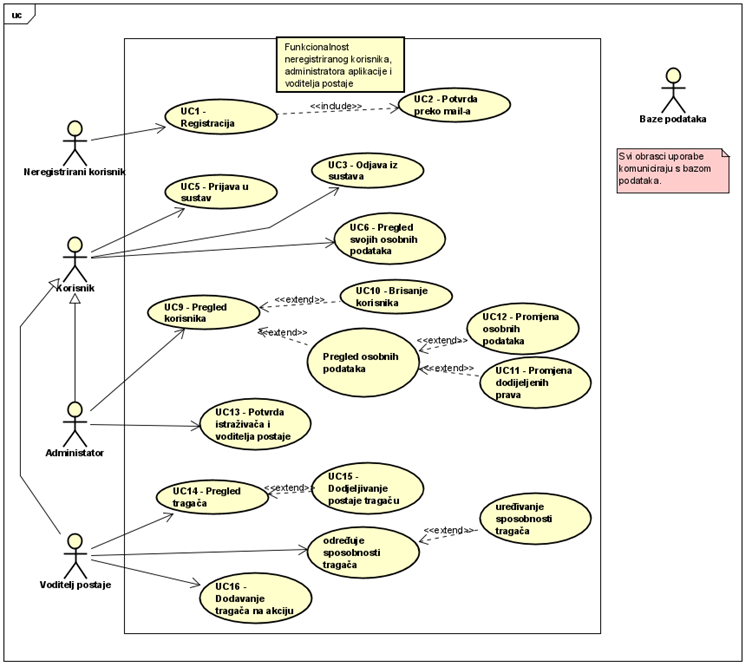
\includegraphics[scale=1]{slike/Funkcionalnost neregistriranog korisnika, administratora aplikacije i voditelja postaje.png} %veličina slike u odnosu na originalnu datoteku i pozicija slike
						\centering
						\caption{Funkcionalnost neregistriranog korisnika, administratora aplikacije i voditelja postaje}
						\label{fig:Funkcionalnost neregistriranog korisnika, administratora aplikacije i voditelja postaje}
					\end{figure}
				
				
					\eject		
				
			\subsection{Sekvencijski dijagrami}
				
				\textbf{\textit{dio 1. revizije}}\\
				
				\textit{Nacrtati sekvencijske dijagrame koji modeliraju najvažnije dijelove sustava (max. 4 dijagrama). Ukoliko postoji nedoumica oko odabira, razjasniti s asistentom. Uz svaki dijagram napisati detaljni opis dijagrama.}
				\eject
	
		\section{Ostali zahtjevi}

		\begin{packed_item}
			\item Sustav treba podržavati istovremeni rad više korisnika u stvarnom vremenu
			\item Korisničko sučelje i sustav moraju podržavati hrvatsku abecedu 
			\item Pristup bazi podataka trebao bi biti učinkovit, s vremenom izvršavanja unutar nekoliko sekundi
			\item Za izradu sustava kao web aplikacije, koriste se objektno-orijentirani jezici
			\item Pogrešna uporaba korisničkog sučelja ne bi smjela imati negativan utjecaj na funkcionalnost i rad sustava
			\item Sustav treba biti jednostavan za korištenje
			\item Pri nadogradnji sustava, ne smiju se narušavati postojeće funkcionalnosti
			\item Veza s bazom podataka mora biti zaštićena, brza i otporna na vanjske greške
			\item Pristup sustavu treba biti moguć iz javne mreže, uz korištenje HTTPS-a radi sigurne komunikacije
		\end{packed_item}
	
	\chapter{Arhitektura i dizajn sustava}

Arhitektura sustava može se podijeliti na tri ključna podsustava:

\begin{packed_enum}
	\item Web poslužitelj:
	\begin{packed_enum}
		\item Ključan dio web aplikacije.
		\item Odgovoran za interakciju između klijenta i aplikacije.
		\item Koristi HTTP/HTTPS protokol za prijenos informacija na webu.
		\item Inicira pokretanje web aplikacije i proslijeđuje zahtjeve.
	\end{packed_enum}
	\item Web aplikacija:
	\begin{packed_enum}
		\item Procesira korisničke zahtjeve i obrađuje ih.
		\item Pristupa bazi podataka prema potrebi.
		\item Generira odgovore u obliku HTML dokumenata za prikaz u web pregledniku.
	\end{packed_enum}			
	\item Baza podataka:	
	\begin{packed_enum}
		\item Sprema podatke koji se koriste ili modificiraju unutar web aplikacije.
	\end{packed_enum}
\end{packed_enum}

Korisnik, putem web preglednika, šalje zahtjeve web poslužitelju. 
Web poslužitelj zatim inicira rad web aplikacije, koja procesira zahtjeve, pristupa bazi podataka po potrebi i vraća odgovore u obliku HTML dokumenata. 
Ova interakcija omogućuje korisnicima pregled i manipulaciju sadržajem putem web sučelja.

\begin{figure}[H]
	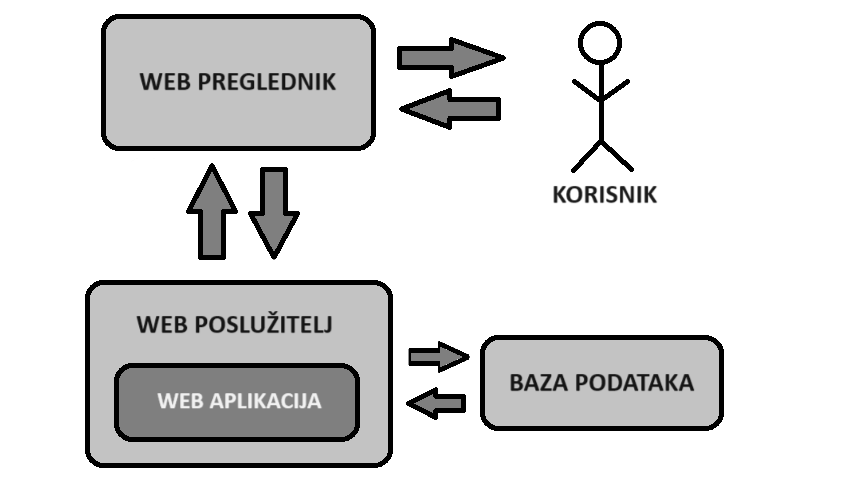
\includegraphics[scale=0.5]{slike/arhitektura.png}
	\centering
	\caption{Arhitektura sustava}
	\label{fig:arhitektura}
\end{figure}

Za izradu ovog projekta koristili smo se Spring Boot frameworkom u Javi kroz
razvojno okruženje IntelliJ Community Edition, Javascriptom uz React u Visual
Studio Code-u te drugim programima za dizajn slika i grafova ( AstahUML itd.).


 Spring Boot podržava koncept MVC, odnosno Model-Pogled-Nadglednik
(engl. \textit{Model View Controller}), arhitekture, tj. stilističke varijacije arhitekture zasnovane 
na događajima. Takve arhitekture odlikuje to što se komponente međusobno ne pozivaju
eksplicitno, već neke od njih generiraju signale (događaje) ne znajući koja druga
"osluškuje" tj. očekuje takav signal i na njega reagira. To se postiže kroz Spring Web MVC modul. 
\begin{packed_item}
	\item Model: Spring Boot omogućava korištenje Java objekata kao modela. Ovi objekti predstavljaju podatke koji se koriste u aplikaciji.
	Spring Data može se integrirati za jednostavno upravljanje podacima i komunikaciju s bazom podataka.
	\item View: Spring Boot pruža fleksibilnost u odabiru tehnologije za prikazivanje korisničkog sučelja. Prikazi se često implementiraju kroz HTML datoteke, a moguće je koristiti različite template engines (Thymeleaf, FreeMarker, JSP).
	Pomoću konfiguracija view resolvera jednostavno se integriraju odabrane tehnologije za prikazivanje podataka korisnicima.
	\item Controller: Anotacije poput @Controller i @RestController omogućuju jednostavno označavanje klasa koje djeluju kao kontroleri.
	@RequestMapping i slične anotacije omogućuju mapiranje HTTP zahtjeva na određene metode kontrolera.
	Spring Boot automatski prepoznaje i konfigurira komponente kontrolera.		
\end{packed_item}

Kod MVC-a pogodno je što smanjuje međuovisnost korisničkog sučelja i ostatka sustava, a omogućuje i nezavisan razvoj, nadogradnje i dodavanje različitih dijelova aplikacije. Sadrži različite
gotove predloške za klase koji nam olakšavaju proces izrade.
				
		\section{Baza podataka}
			    


		Baze podataka neizostavan su dio razvoja programske potpore jer danas gotova svaka domena primjene 
		obiluje mnoštvom podataka koje treba pohraniti na organiziran način kako bi se efikasno dohvaćali,
		 mijenjali i nadopunjavali. Za upravljanje bazom podataka mogu se koristiti različiti sustavi koji 
		 obavljaju optimiranje upita i omogućuju rukovanje podatcima. Mi smo odlučili koristiti PostgreSQL 
		 koji nam je bio preporučen na kolegiju Baze podataka. \newline Relacijski nam model baze podataka 
		 omogućuje vjeran prikaz stvarnosti pomoću relacija u koje pohranjujemo vrijednosti odabranih 
		 atributa vezanih uz entitete bitne za domenu primjene. Atributi su imenovani stupci te tablice. ER (Entity-Relationship) model podataka zadržava dobra svojstva relacijskog modela, a uz to omogućuje eksplicitni prikaz semantičkih informacija vezanih uz veze (odnose) između entiteta. Kako bismo prikazali kako su eniteti našeg sustava povezani koristit ćemo ER model baze podataka.
za podataka ove aplikacije sastoji se od sljedećih entiteta:
		\begin{packed_item}
			\item Korisnik
			\item Pozicija tragača
			\item Uloga
			\item Zadatak 
			\item Pripada postaji
			\item Osposobljen za
			\item Akcija
			\item Postaja
			\item Prijevozno sredstvo
			\item Komentar korisnika 
			\item Životinja
			\item Pozicija životinje
		\end{packed_item}

		\eject
			\subsection{Opis tablica}
			
					\textbf {Zadatak} Ovaj entitet sadrži sve važne informacije o zadatcima koje obavljaju tragači tijekom akcije, a stvaraju istraživači. Sadrži
				atribute: šifra zadatka, korisničko ime, tekst, završen, šifra akcije, šifra životinje i šifra vozila. 
				Ova tablica je u vezi s tablicom Prijevozno sredstvo preko tablice Osposobljen za te izravno preko 
				dentifikatora vozila(šifra vozila), s tablicom Akcija izravno preko identifikatora akcije (šifra akcije), 
				s tablicom Životinja izravno preko identifikatora životinje (šifra životinje).
				
				\begin{longtblr}[
					label=none,
					entry=none
					]{
						width = \textwidth,
						colspec={|X[6,l]|X[6, l]|X[20, l]|}, 
						rowhead = 1,
					} %definicija širine tablice, širine stupaca, poravnanje i broja redaka naslova tablice
					\hline \SetCell[c=3]{c}{\textbf{Zadatak}}	 \\ \hline[3pt]
					\SetCell{LightGreen} Šifra Zadatka & INT	&  	Jedinstveni brojčani identifikator zadatka  	\\ \hline
					\SetCell{LightGreen} Korisničko ime & VARCHAR	& 	Korisničko ime korisnika\\ \hline
					Tekst	& VARCHAR & Opis zadatka  	\\ \hline 
					Završen & BOOLEAN & Status je li zadatak završen  \\ \hline 
          \SetCell{LightBlue} Šifra akcije 	& INT & Jedinstveni brojčani identifikator akcije   	\\ \hline 
          \SetCell{LightBlue} Šifra životinje 	& INT &   Jedinstveni brojčani identifikator životinje  	\\ \hline 
          \SetCell{LightBlue} Šifra vozila 	& INT &  Jedinstveni brojčani identifikator vozila 	\\ \hline 
				\end{longtblr}

				\textbf {Akcija} Ovaj entitet sadrži sve važne informacije o akcijama pretraživanja i praćenja. Sadrži
			atribute: šifra akcije, naziv akcije, aktivna i korisničko ime. 
			Ova tablica je u vezi s tablicom Korisnik preko identifikatora korisnika(korisničko ime),
			 s tablicom Životinja preko tablice Komentar korisnika, s tablicom Zadatak i tablicom Pozicija tragača.
				
				\begin{longtblr}[
					label=none,
					entry=none
					]{
						width = \textwidth,
						colspec={|X[6,l]|X[6, l]|X[20, l]|}, 
						rowhead = 1,
					} %definicija širine tablice, širine stupaca, poravnanje i broja redaka naslova tablice
          \hline \SetCell[c=3]{c}{\textbf{Akcija}}	 \\ \hline[3pt]
					\SetCell{LightGreen} Šifra akcije & INT	&  	Jedinstveni ključ za identifikaciju zadatka  	\\ \hline
					Naziv akcije	& VARCHAR &  Puni naziv akcije  	\\ \hline 
					Aktivna & BOOLEAN & Status je li akcija aktvna  \\ \hline 
          \SetCell{LightBlue} Korisničko ime 	& VARCHAR &  Korisničko ime korisnika 	\\ \hline 
				\end{longtblr}
			
				\textbf {Komentar korisnika} Ovaj entitet sadrži informacije o komentarima korisnika o praćenoj životinji 
				koje mogu ostaviti tijekom akcije. Sadrži atribute: šifra životinje, korisničko ime, šifra akcije i komentar. 
		

				\begin{longtblr}[
					label=none,
					entry=none
					]{
						width = \textwidth,
						colspec={|X[6,l]|X[6, l]|X[20, l]|}, 
						rowhead = 1,
					} %definicija širine tablice, širine stupaca, poravnanje i broja redaka naslova tablice
          \hline \SetCell[c=3]{c}{\textbf{Komentar korisnika}}	 \\ \hline[3pt]
					\SetCell{LightGreen} Šifra životinje & INT	&  	Jedinstveni brojčani identifikator zadatka  	\\ \hline
					\SetCell{LightGreen} Korisničko ime & VARCHAR	&  	Korisničko ime korisnika 	\\ \hline
					\SetCell{LightGreen} Šifra akcije & INT	&  	Jedinstveni brojčani identifikator akcije  	\\ \hline
					Komentar	& VARCHAR & Sadržaj komentara  	\\ \hline 
				\end{longtblr}
				
				\textbf {Životinja} Ovaj entitet sadrži sve važne informacije o životinjama. Sadrži
			atribute: šifra životinje, naziv , latinski naziv i opis. 
			Ova tablica povezana je s tablicom Pozicija životinje s tablicom Zadatak preko identifikatora životinje(šifra životinje) te s tablicom Akcija

				\begin{longtblr}[
					label=none,
					entry=none
					]{
						width = \textwidth,
						colspec={|X[6,l]|X[6, l]|X[20, l]|}, 
						rowhead = 1,
					} %definicija širine tablice, širine stupaca, poravnanje i broja redaka naslova tablice
          \hline \SetCell[c=3]{c}{\textbf{Životinja}}	 \\ \hline[3pt]
					\SetCell{LightGreen} Šifra životinje & INT	&  	Jedinstveni brojčani identifikator životinje  	\\ \hline
					Naziv	& VARCHAR & Puni naziv životinje  	\\ \hline 
					Latinski naziv	& VARCHAR & Latinski naziv životinje  	\\ \hline 
					Opis	& VARCHAR & Sadržaj komentara  	\\ \hline 
				\end{longtblr}

				\textbf {Pozicija životinje} Ovaj entitet sadrži informacije o poziciji životinje. 
				Pomoću njega bilježimo gibanje životinje na kartama. Sadrži
			atribute: šifra životinje, vremenska oznaka, geografska širina i geografska dužina.


				\begin{longtblr}[
					label=none,
					entry=none
					]{
						width = \textwidth,
						colspec={|X[6,l]|X[6, l]|X[20, l]|}, 
						rowhead = 1,
					} %definicija širine tablice, širine stupaca, poravnanje i broja redaka naslova tablice
          \hline \SetCell[c=3]{c}{\textbf{Pozicija životinje}}	 \\ \hline[3pt]
					\SetCell{LightGreen} Šifra životinje & INT	&  	Jedinstveni brojčani identifikator životinje \\ \hline
					\SetCell{LightGreen} Vremenska oznaka & TIMESTAMP	&  	Zadnje vrijeme u kojem je viđena životinja  	\\ \hline
          Geografska širina	& DOUBLE & Iznos geografske širine  	\\ \hline 
          Geografska dužina	& DOUBLE & Iznos geografske dužine  	\\ \hline 
				\end{longtblr}

				\textbf {Pozicija tragača} Ovaj entitet sadrži informacije o poziciji tragača. 
				Pomoću njega bilježimo kretanje tragača na kartama. Sadrži
			atribute: korisničko ime, vremenska oznaka, šifra akcije, geografska širina i geografska dužina.

				\begin{longtblr}[
					label=none,
					entry=none
					]{
						width = \textwidth,
						colspec={|X[6,l]|X[6, l]|X[20, l]|}, 
						rowhead = 1,
					} %definicija širine tablice, širine stupaca, poravnanje i broja redaka naslova tablice
          \hline \SetCell[c=3]{c}{\textbf{Pozicija tragača}}	 \\ \hline[3pt]
					\SetCell{LightGreen} Korisničko ime & VARCHAR	&  	Korisničko ime korisnika  	\\ \hline
					\SetCell{LightGreen} Vremenska oznaka & TIMESTAMP	&  	Zadnje vrijeme kada je tragač zabilježio svoju poziciju  	\\ \hline
					\SetCell{LightGreen} Šifra akcije & INT	&  	Jedinstveni brojčani identifikator akcije  	\\ \hline
          Geografska širina	& DOUBLE & Iznos geografske širine  	\\ \hline 
          Geografska dužina	& DOUBLE & Iznos geografske dužine  	\\ \hline 
				\end{longtblr}

				\textbf {Korisnik} Ovaj entitet sadrži sve važne informacije o korisnicima. Sadrži
			atribute: korisničko ime, email, lozinka, ime, prezime, fotografija i šifra uloge.
			Ova tablica je u vezi s tablicama Akcija, Pozicija tragača, Uloga i Komentar korisnika.

				\begin{longtblr}[
					label=none,
					entry=none
					]{
						width = \textwidth,
						colspec={|X[6,l]|X[6, l]|X[20, l]|}, 
						rowhead = 1,
					} %definicija širine tablice, širine stupaca, poravnanje i broja redaka naslova tablice
          \hline \SetCell[c=3]{c}{\textbf{Korisnik}}	 \\ \hline[3pt]
					\SetCell{LightGreen} Korisničko ime & VARCHAR	&  	Ime korisnika  	\\ \hline
          Email	& VARCHAR & Sadržaj komentara  	\\ \hline 
          Lozinka & VARCHAR & Lozinka korisnika \\ \hline
          Ime & VARCHAR & Ime korisnika \\ \hline
          Prezime & VARCHAR & Prezime korisnika \\ \hline
          Fotografija & VARCHAR & Fotografija korisnika \\ \hline
          \SetCell{LightBlue} Šifra uloge 	& INT &   Jedinstveni brojčani identifikator uloge	\\ \hline 

				\end{longtblr}

				\textbf {Pripada postaji} Ova veza sadrži informacije po kojima saznajemo koji korisnik pripada kojoj postaji.
				Povezuje entitete Korisnik i Postaja te sadrži njihove ključne atribute: korisničko ime i šifra postaje.

				\begin{longtblr}[
					label=none,
					entry=none
					]{
						width = \textwidth,
						colspec={|X[6,l]|X[6, l]|X[20, l]|}, 
						rowhead = 1,
					} %definicija širine tablice, širine stupaca, poravnanje i broja redaka naslova tablice
          \hline \SetCell[c=3]{c}{\textbf{Pripada postaji}}	 \\ \hline[3pt]
					\SetCell{LightGreen} Korisničko ime & VARCHAR	&  	Korisničko ime korisnika  	\\ \hline
					\SetCell{LightGreen} Šifra postaje & VARCHAR	&  	Jedinstveni brojčani identifikator postaje\\ \hline

				\end{longtblr}

				\textbf {Postaja} Ovaj entitet sadrži informacije o postajama. Sastoji se od
			atributa: šifra postaje i naziv postaje.

				\begin{longtblr}[
					label=none,
					entry=none
					]{
						width = \textwidth,
						colspec={|X[6,l]|X[6, l]|X[20, l]|}, 
						rowhead = 1,
					} %definicija širine tablice, širine stupaca, poravnanje i broja redaka naslova tablice
          \hline \SetCell[c=3]{c}{\textbf{Postaja}}	 \\ \hline[3pt]
					\SetCell{LightGreen} Šifra postaje & VARCHAR	&  	Jedinstveni brojčani identifikator korisnika \\ \hline
					Naziv postaje & VARCHAR	&  	Pun naziv postaje  	\\ \hline

				\end{longtblr}

				\textbf {Osposobljen za} Ova veza sadrži informacije po kojima saznajemo koji korisnik ima sposobnosti za voziti koje prijevozno sredstvo.
				Povezuje entitete Korisnik i Prijevozno sredstvo te sadrži njihove ključne atribute: korisničko ime i šifra vozila.

				\begin{longtblr}[
					label=none,
					entry=none
					]{
						width = \textwidth,
						colspec={|X[6,l]|X[6, l]|X[20, l]|}, 
						rowhead = 1,
					} %definicija širine tablice, širine stupaca, poravnanje i broja redaka naslova tablice
          \hline \SetCell[c=3]{c}{\textbf{Osposobljen za}}	 \\ \hline[3pt]
					\SetCell{LightGreen} Korisničko ime & VARCHAR	&  	Ime korisnika  	\\ \hline
					\SetCell{LightGreen} Šifra vozila & INT	&   Jedinstveni brojčani identifikator vozila  	\\ \hline

				\end{longtblr}

				\textbf {Prijevozno sredstvo} Ovaj entitet sadrži informacije o vozilima za koje tragači mogu biti osposobljeni.
				 Sastoji se od atributa: šifra vozila i naziv vozila.


				\begin{longtblr}[
					label=none,
					entry=none
					]{
						width = \textwidth,
						colspec={|X[6,l]|X[6, l]|X[20, l]|}, 
						rowhead = 1,
					} %definicija širine tablice, širine stupaca, poravnanje i broja redaka naslova tablice
          \hline \SetCell[c=3]{c}{\textbf{Prijevozno sredstvo}}	 \\ \hline[3pt]
					\SetCell{LightGreen} Šifra vozila & INT	&   Jedinstveni brojčani identifikator vozila  	\\ \hline
          Naziv vozila & VARCHAR & Puni naziv vozila \\ \hline

				\end{longtblr}

				\textbf {Uloga} Ovaj entitet sadrži informacije o ulogama korisnika. Sastoji se od
			atributa: šifra uloge i naziv uloge.


				\begin{longtblr}[
					label=none,
					entry=none
					]{
						width = \textwidth,
						colspec={|X[6,l]|X[6, l]|X[20, l]|}, 
						rowhead = 1,
					} %definicija širine tablice, širine stupaca, poravnanje i broja redaka naslova tablice
          \hline \SetCell[c=3]{c}{\textbf{Uloga}}	 \\ \hline[3pt]
          \SetCell{LightGreen} Šifra Uloge & INT	&  Jedinstveni brojčani identifikator uloge	\\ \hline
          Naziv uloge	& VARCHAR & Puni naziv uloge  	\\ \hline 

				\end{longtblr}

			\eject

			\subsection{Dijagram baze podataka}

			\begin{figure}[H]
				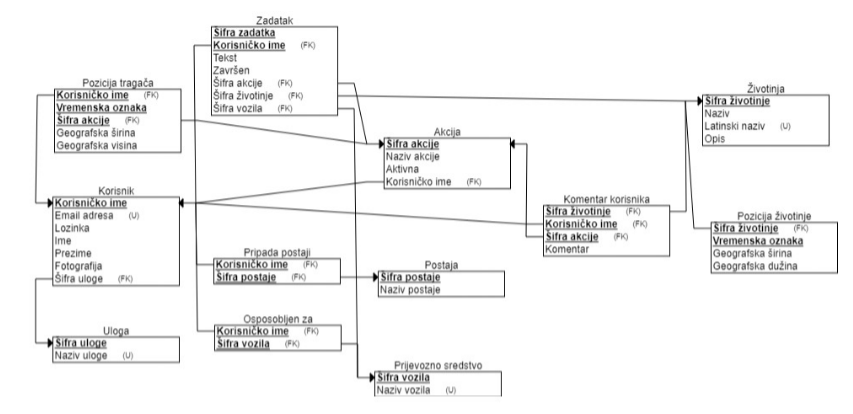
\includegraphics[scale=0.9]{slike/dijagram baze podataka.png} 
				\centering
				\caption{Dijagram baze podataka}
				\label{fig:dijagram_baze_podataka}
			\end{figure}
			
			\eject
			
			
		\section{Dijagram razreda}

		Na slikama \ref{fig:controllers}, \ref{fig:data_transfer_objects} i \ref{fig:models} su prikazani klasni dijagrami koji pripadaju backend dijelu MVC
		arhitekture. Razredi prikazani na slici \ref{fig:controllers} nasljeđuju Controller razred. 
		Metode implementirane u tim razredima manipuliraju s Data transfer object, a oni
		su dohvaćeni s pomoću metoda u Model razredima. 

		Metode unutar Controller razreda vraćaju JSON datoteke s odgovarajućim html status kodom.
		Razredi su logički podijeljeni prema pravu pristupa metodama specifičnih aktora kako bi se smanjila prenapučenost unutar dijagrama.
		Pri prikazu su naglašene samo ovisnosti između razreda koji pripadaju istom dijelu dijagrama radi jednostavnije organizacije.
		Vrsta ovisnosti između različitim razredima može se zaključiti iz naziva i tipova atributa unutar tih razreda.
		
		\eject

			\begin{figure}[H]
				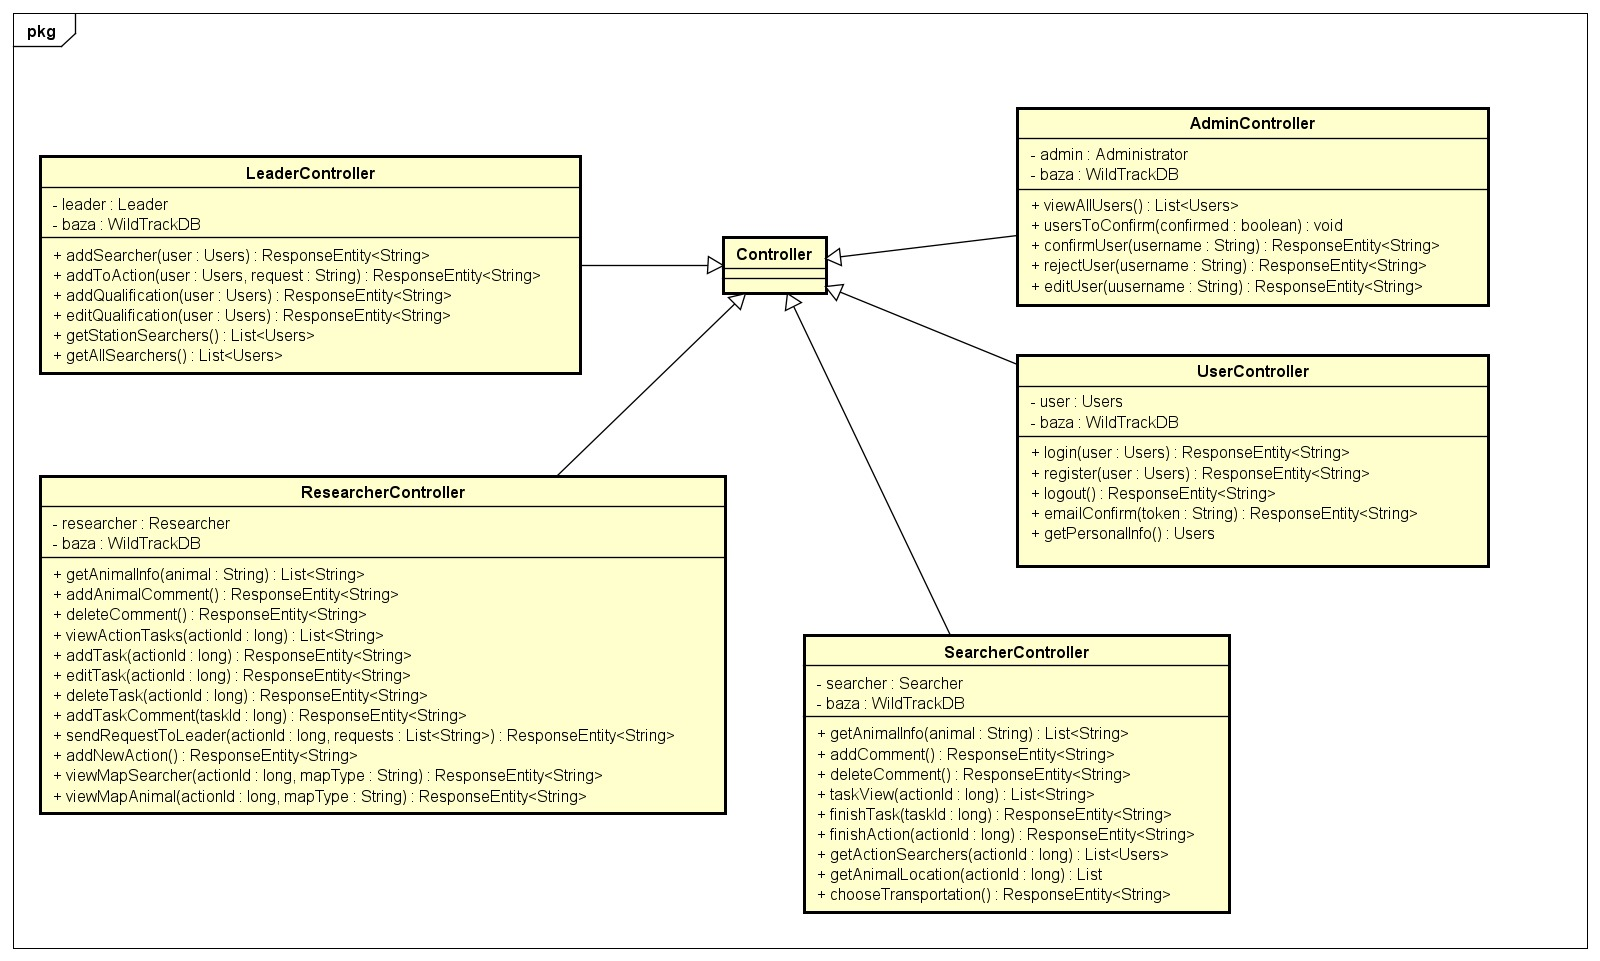
\includegraphics[scale=0.4]{slike/klasni_dijagram_controllers.jpg}
				\centering
				\caption{Dijagram razreda - dio Controllers}
				\label{fig:controllers}
			\end{figure}
			
			\eject

			\begin{figure}[H]
				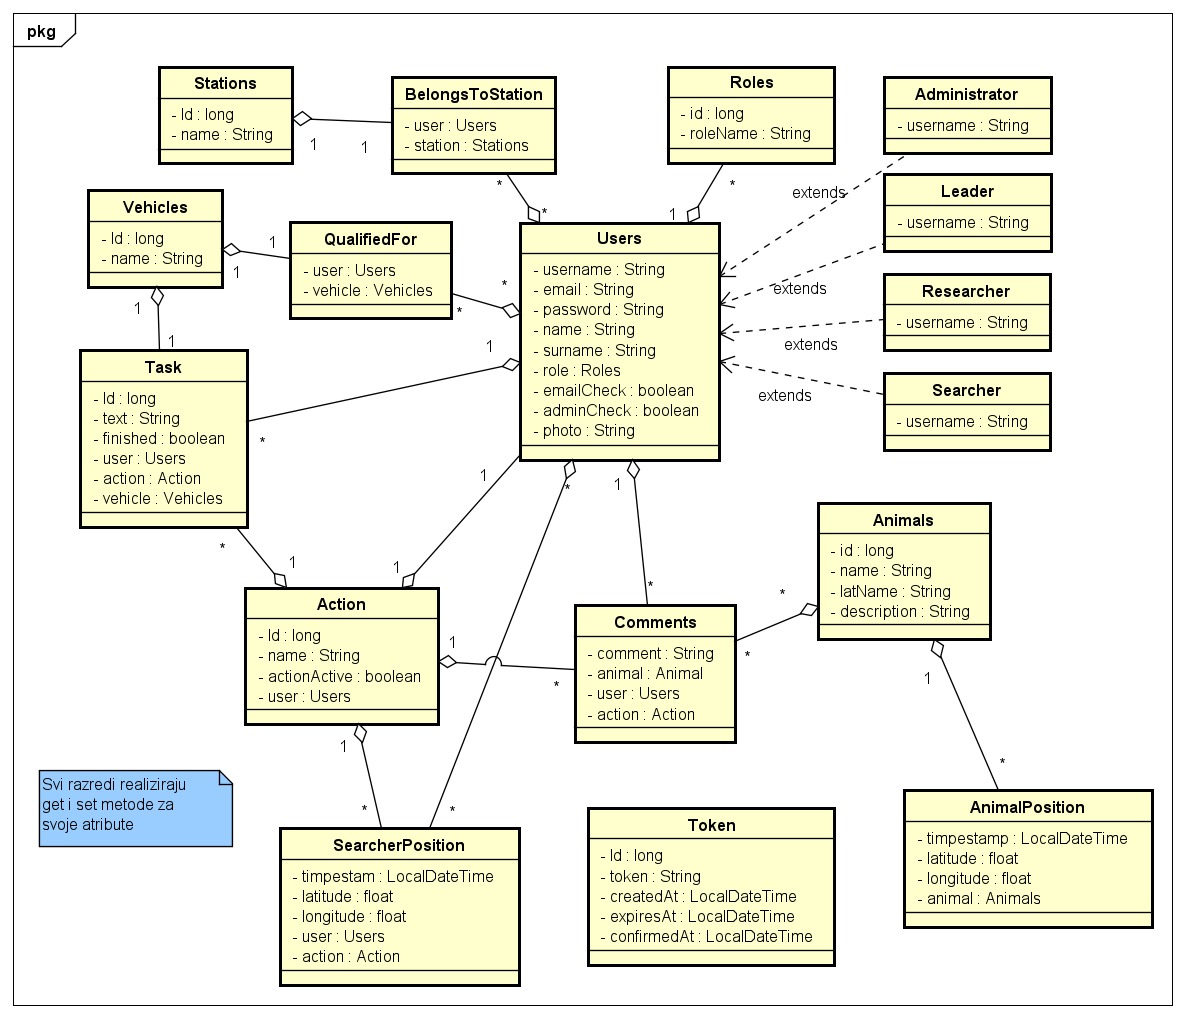
\includegraphics[scale=0.5]{slike/klasni_dijagram_data_transfer_objects.jpg}
				\centering
				\caption{Dijagram razreda - dio Data transfer objects}
				\label{fig:data_transfer_objects}
			\end{figure}

			Model razredi prikazuju strukturu baze podataka u aplikaciji. 
			Implementirane metode komuniciraju s bazom podataka te vraćaju tražene podatke. 
			Razred Users predstavlja neregistriranog korisnika koji se može registrirati u 
			sustav unošenjem informacija. Razred Administrator predstavlja administratora 
			sustava koji ima najveće ovlasti. Razred Leader predstavlja voditelja postaje koji ima mogućnost postavljanja tragača određenom istraživaču.
			Razred Researcher predstavlja istraživača koji ima pristup karti tragača i životinja te može tragaču zadati zadatak. 
			Razred Searcher predstavlja tragača koji ima pristup karti životinja te može ispunjavati zadatke.


			\eject

			\begin{figure}[H]
				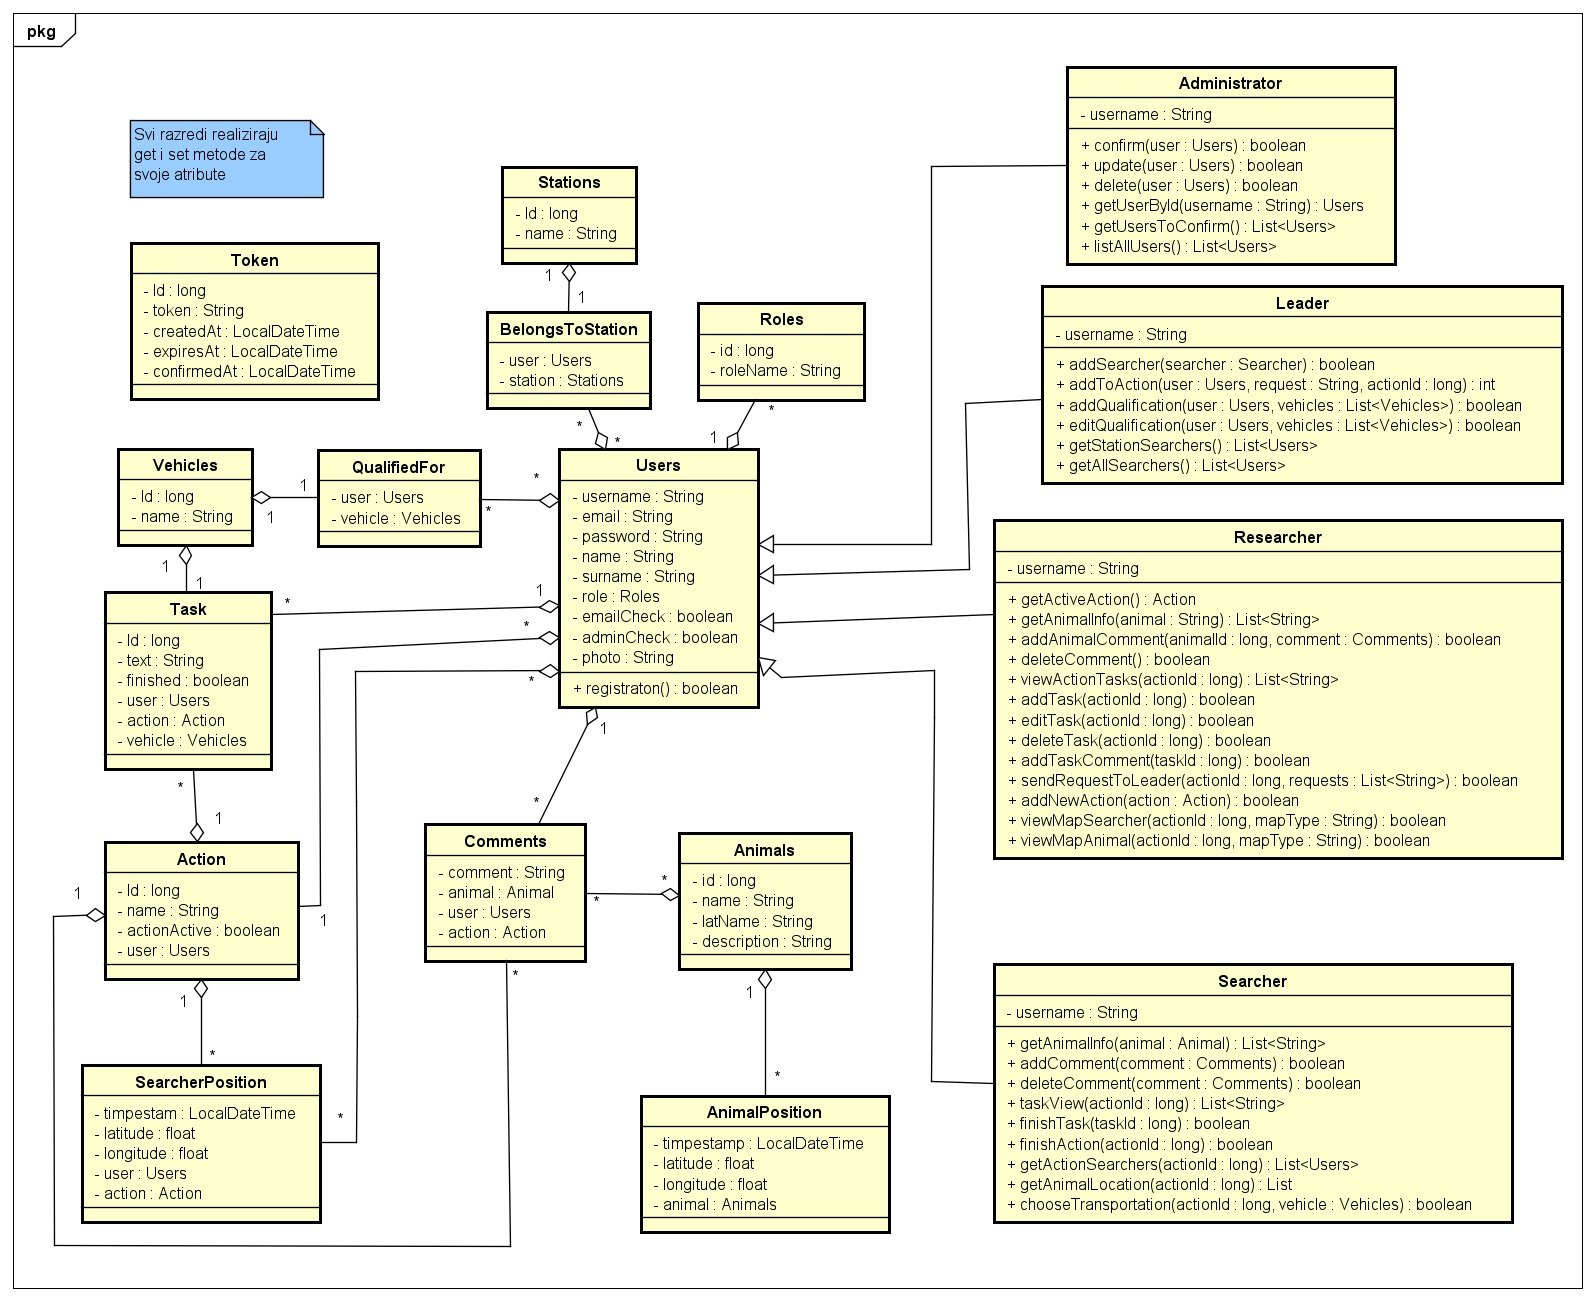
\includegraphics[scale=0.4]{slike/klasni_dijagram_models.jpg}
				\centering
				\caption{Dijagram razreda - dio Models}
				\label{fig:models}
			\end{figure}
			

			\textbf{\textit{dio 2. revizije}}\\			
			
			\textit{Prilikom druge predaje projekta dijagram razreda i opisi moraju odgovarati stvarnom stanju implementacije}
			
			
			
			\eject
		
		\section{Dijagram stanja}
			
			Dijagram stanja (slika \ref{fig:dijagram stanja - tragač}) opisuje dinamičko ponašanje sustava uslijed raznih mogućih
		događaja. Uspješnom prijavom prikazana je početna stranica korisnika u ulozi tragača. 
		Na početnoj stranici tragač bira jednu od tri opcije:
		\begin{packed_item}
		\item opciju \textit{Moj profil} dostupnu svakom korisniku, koja ga vodi na stranicu sa osobnim podacima, gdje ih može uređivati
		\item opciju \textit{O životinjama} koja ga vodi na stranicu na kojoj su prikazane sve vrste životinja u aplikaciji, a klikom na pojedinu vrstu dobiva popis jedinki te vrste i dalje klikom na pojedinu jedinku dobiva opširnije informacije specifično o toj jedinki
		\item opciju \textit{Moja akcija} koja ga vodi na stranicu s prikazom karte i dodatnim opcijama za pregled zadataka, ostalih tragača i praćenih životinja; nakon klika na praćene životinje ili ostale tragače, tragaču se prikazuje lista istih, a klikom na pojedinca te liste(tragača ili životinju) na karti mu se prikazuje trenutna pozicija odabranog
		\end{packed_item}

		\begin{figure}[H]
			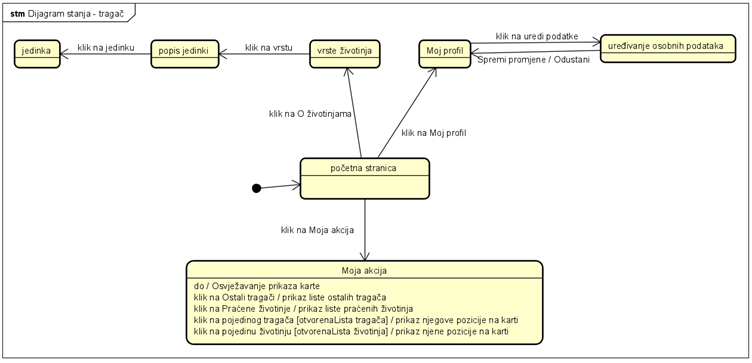
\includegraphics[scale=0.5]{slike/dijagram stanja - tragač.png}
			\centering
			\caption{Dijagram stanja - tragač}
			\label{fig:dijagram stanja - tragač}
		\end{figure}
			
			\eject 
		
		\section{Dijagram aktivnosti}

		Dijagramom aktivnosti na slici  \ref{fig:dijagram aktivnosti - stvaranje nove akcije} modelirano je stvaranje nove akcije korisnika u ulozi istraživača.
		Do postupka stvaranja nove akcije dolazi se sa stranice prikaza popisa akcija klikom na 
		\textit{Stvori novu akciju}. Na formularu za novu akciju se prilikom klika na \textit{Stvori novu akciju},
		prije spremanja podataka nove akcije u bazu, provjerava jesu li uneseni svi potrebni podatci i jesu li uneseni podatci ispravni.
		Nakon uspješnog stvaranja nove akcije, korisniku se prikazuje osvježen popis akcija, a ukoliko korisnik odustane od stvaranja nove akcije klikom na 
		\textit{Odustani} prikaz se vraća na popis akcija.

		\begin{figure}[H]
			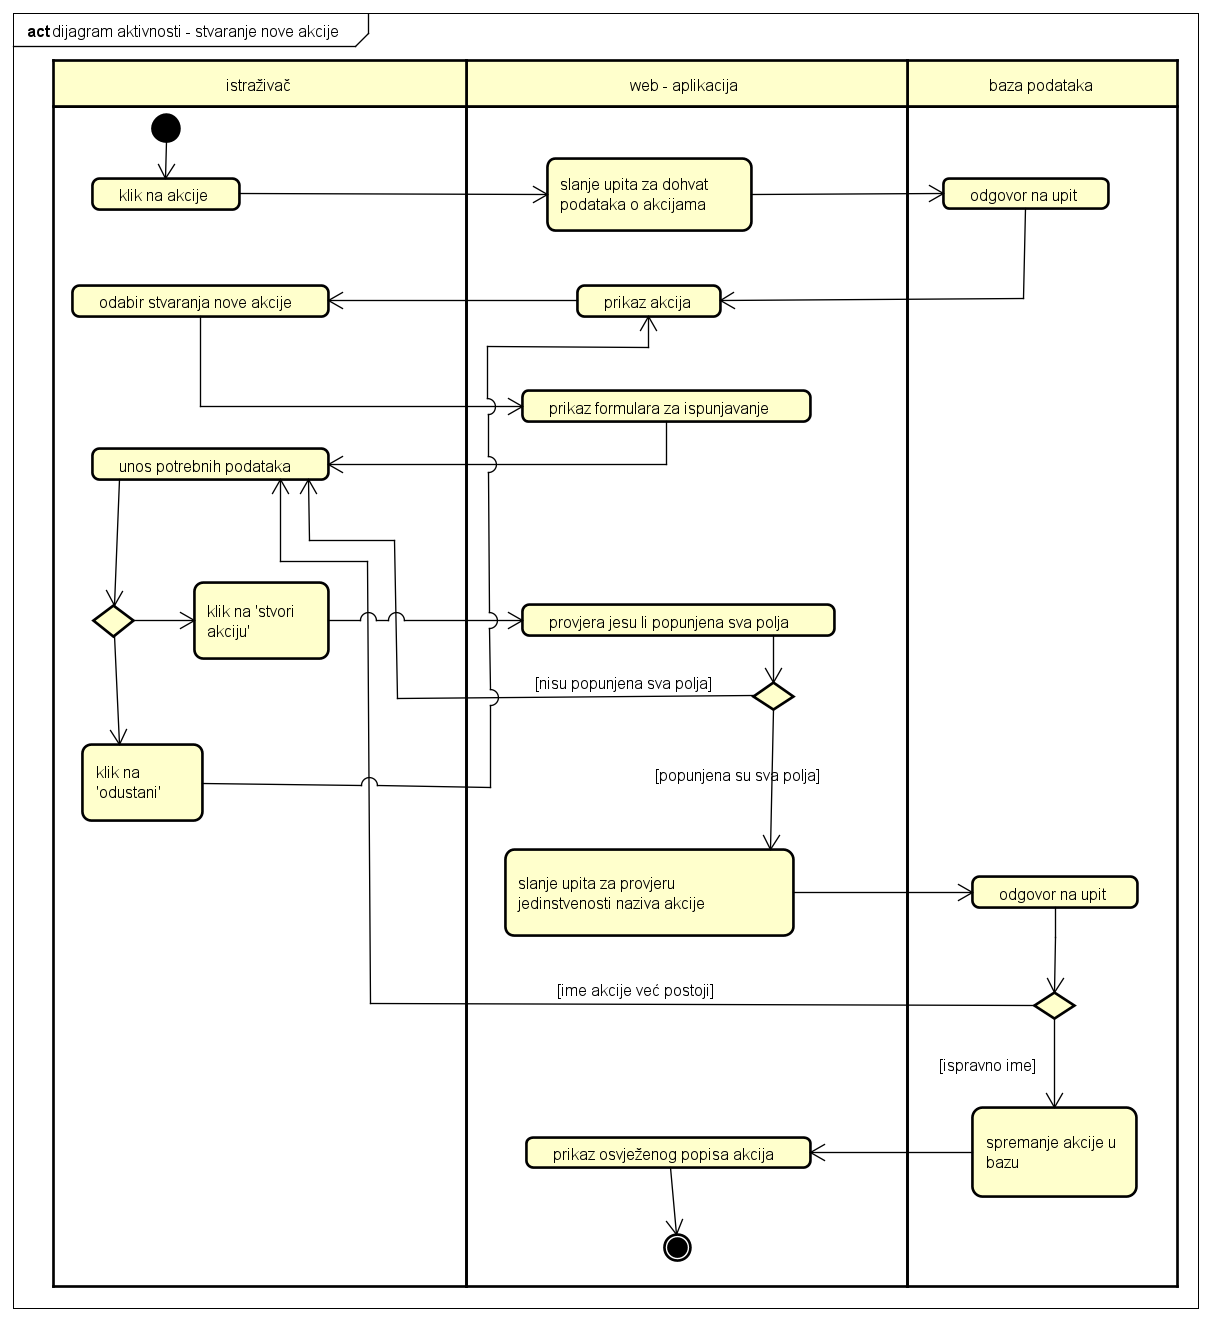
\includegraphics[scale=0.5]{slike/dijagram aktivnosti - stvaranje nove akcije.png}
			\centering
			\caption{Dijagram aktivnosti - stvaranje nove akcije}
			\label{fig:dijagram aktivnosti - stvaranje nove akcije}
		\end{figure}

			\eject
		\section{Dijagram komponenti}
		
			\textbf{\textit{dio 2. revizije}}\\
		
			 \textit{Potrebno je priložiti dijagram komponenti s pripadajućim opisom. Dijagram komponenti treba prikazivati strukturu cijele aplikacije.}

	\chapter{Implementacija i korisničko sučelje}
		
		
		\section{Korištene tehnologije i alati}
		
			
			  U izradi projekta većina digitalne komunikacije ostvarena je preko platforme
			  \textbf{WhatsApp} (\textit{https://web.whatsapp.com/} ).

			  Korištene su sljedeće tehnologije i alati:

			  \begin{packed_item}

				\item \textbf{Springboot}
					\begin{packed_item}
						\item open source radni okvir za kreaciju mikro-servisa, idealan za potrebe projekta
						\item u njemu je izrađen backend dio projekta 
						\item \textit{https://spring.io/projects/spring-boot}
					\end{packed_item}

				\item \textbf{React}
				\begin{packed_item}
					\item JavaScript biblioteka za izgradnju korisničkih sučelja 
					\item korišten za izradu čitavog frontenda dijela aplikacije s kojim korisnik dolazi u interakciju 
					\item provjerava ispravnost podataka unesenih u obrasce 
					\item \textit{ https://www.reactjs.org/}
				\end{packed_item}

				\item \textbf{PostgreSQL }
				\begin{packed_item}
					\item jezik u kojem je napravljena baza podataka  
					\item besplatan i open source sustav za upravljanje relacijskim bazama podataka s naglaskom na mogućnosti proširivanja  
					\item \textit{ https://www.postgresql.org/}
				\end{packed_item}
				
				\item \textbf{pgAdmin}
				\begin{packed_item}
					\item za upravljanje bazom podataka neovisno o backendu 
					\item \textit{ https://www.pgadmin.org/}
				\end{packed_item}

				\item \textbf{IntelliJ }
				\begin{packed_item}
					\item  IDE za javu u kojem je kodiran backend dio projekta 
					\item \textit{ https://www.jetbrains.com/idea/}
				\end{packed_item}

				\item \textbf{Visual Studio Code}
				\begin{packed_item}
					\item  uređivač izvornog koda za razne programske jezike
					\item  korišten za kodiranje frontend dijela projekta i projektne dokumentacije
					\item \textit{ https://code.visualstudio.com/}
				\end{packed_item}

				\item \textbf{Astah UML }
				\begin{packed_item}
					\item program za uređivanje svih vrsta UML dijagrama
					\item svi dijagrami u ovom dokumentu izrađeni su u Astahu 
					\item \textit{https://astah.net/products/astah-uml/}
				\end{packed_item}

				\item \textbf{GitHub }
				\begin{packed_item}
					\item  stranica za funkcionalno zajedničko stvaranje i uređivanje grupnog projekta 
					\item \textit{https://github.com/}
				\end{packed_item}

				\item \textbf{Latex}
				\begin{packed_item}
					\item programski jezik za pisanje strukturiranih tekstova, često korišten za stvaranje profesionalnih dokumenata
					\item koristi markup jezik koji prevodi u formatirane dokumente
					\item korišten za dokumentiranje projekta
					\item \textit{https://www.latex-project.org/}
				\end{packed_item}
			\end{packed_item}
			
			 \eject 
		
	
		\section{Ispitivanje programskog rješenja}
			
			\textbf{\textit{dio 2. revizije}}\\
			
			 \textit{U ovom poglavlju je potrebno opisati provedbu ispitivanja implementiranih funkcionalnosti na razini komponenti i na razini cijelog sustava s prikazom odabranih ispitnih slučajeva. Studenti trebaju ispitati temeljnu funkcionalnost i rubne uvjete.}
	
			
			\subsection{Ispitivanje komponenti}
			\textit{Potrebno je provesti ispitivanje jedinica (engl. unit testing) nad razredima koji implementiraju temeljne funkcionalnosti. Razraditi \textbf{minimalno 6 ispitnih slučajeva} u kojima će se ispitati redovni slučajevi, rubni uvjeti te izazivanje pogreške (engl. exception throwing). Poželjno je stvoriti i ispitni slučaj koji koristi funkcionalnosti koje nisu implementirane. Potrebno je priložiti izvorni kôd svih ispitnih slučajeva te prikaz rezultata izvođenja ispita u razvojnom okruženju (prolaz/pad ispita). }
			
			
			
			\subsection{Ispitivanje sustava}
			
			 \textit{Potrebno je provesti i opisati ispitivanje sustava koristeći radni okvir Selenium\footnote{\url{https://www.seleniumhq.org/}}. Razraditi \textbf{minimalno 4 ispitna slučaja} u kojima će se ispitati redovni slučajevi, rubni uvjeti te poziv funkcionalnosti koja nije implementirana/izaziva pogrešku kako bi se vidjelo na koji način sustav reagira kada nešto nije u potpunosti ostvareno. Ispitni slučaj se treba sastojati od ulaza (npr. korisničko ime i lozinka), očekivanog izlaza ili rezultata, koraka ispitivanja i dobivenog izlaza ili rezultata.\\ }
			 
			 \textit{Izradu ispitnih slučajeva pomoću radnog okvira Selenium moguće je provesti pomoću jednog od sljedeća dva alata:}
			 \begin{itemize}
			 	\item \textit{dodatak za preglednik \textbf{Selenium IDE} - snimanje korisnikovih akcija radi automatskog ponavljanja ispita	}
			 	\item \textit{\textbf{Selenium WebDriver} - podrška za pisanje ispita u jezicima Java, C\#, PHP koristeći posebno programsko sučelje.}
			 \end{itemize}
		 	\textit{Detalji o korištenju alata Selenium bit će prikazani na posebnom predavanju tijekom semestra.}
			
			\eject 
		
		
		\section{Dijagram razmještaja}
			
			\textbf{\textit{dio 2. revizije}}
			
			 \textit{Potrebno je umetnuti \textbf{specifikacijski} dijagram razmještaja i opisati ga. Moguće je umjesto specifikacijskog dijagrama razmještaja umetnuti dijagram razmještaja instanci, pod uvjetom da taj dijagram bolje opisuje neki važniji dio sustava.}
			
			\eject 
		
		\section{Upute za puštanje u pogon}
		
			\textbf{\textit{dio 2. revizije}}\\
		
			 \textit{U ovom poglavlju potrebno je dati upute za puštanje u pogon (engl. deployment) ostvarene aplikacije. Na primjer, za web aplikacije, opisati postupak kojim se od izvornog kôda dolazi do potpuno postavljene baze podataka i poslužitelja koji odgovara na upite korisnika. Za mobilnu aplikaciju, postupak kojim se aplikacija izgradi, te postavi na neku od trgovina. Za stolnu (engl. desktop) aplikaciju, postupak kojim se aplikacija instalira na računalo. Ukoliko mobilne i stolne aplikacije komuniciraju s poslužiteljem i/ili bazom podataka, opisati i postupak njihovog postavljanja. Pri izradi uputa preporučuje se \textbf{naglasiti korake instalacije uporabom natuknica} te koristiti što je više moguće \textbf{slike ekrana} (engl. screenshots) kako bi upute bile jasne i jednostavne za slijediti.}
			
			
			 \textit{Dovršenu aplikaciju potrebno je pokrenuti na javno dostupnom poslužitelju. Studentima se preporuča korištenje neke od sljedećih besplatnih usluga: \href{https://aws.amazon.com/}{Amazon AWS}, \href{https://azure.microsoft.com/en-us/}{Microsoft Azure} ili \href{https://www.heroku.com/}{Heroku}. Mobilne aplikacije trebaju biti objavljene na F-Droid, Google Play ili Amazon App trgovini.}
			
			
			\eject 
	\chapter{Zaključak i budući rad}
		
		\textbf{\textit{dio 2. revizije}}\\
		
		 \textit{U ovom poglavlju potrebno je napisati osvrt na vrijeme izrade projektnog zadatka, koji su tehnički izazovi prepoznati, jesu li riješeni ili kako bi mogli biti riješeni, koja su znanja stečena pri izradi projekta, koja bi znanja bila posebno potrebna za brže i kvalitetnije ostvarenje projekta i koje bi bile perspektive za nastavak rada u projektnoj grupi.}
		
		 \textit{Potrebno je točno popisati funkcionalnosti koje nisu implementirane u ostvarenoj aplikaciji.}
		
		\eject 
	\chapter*{Popis literature}
		\addcontentsline{toc}{chapter}{Popis literature}
	 	
 		\textbf{\textit{Kontinuirano osvježavanje}}
	
		\textit{Popisati sve reference i literaturu koja je pomogla pri ostvarivanju projekta.}
		
		
		\begin{enumerate}
			
			
			\item  Programsko inženjerstvo, FER ZEMRIS, \url{http://www.fer.hr/predmet/proinz}
			
			\item  I. Sommerville, "Software engineering", 8th ed, Addison Wesley, 2007.
			
			\item  T.C.Lethbridge, R.Langaniere, "Object-Oriented Software Engineering", 2nd ed. McGraw-Hill, 2005.
			
			\item  I. Marsic, Software engineering book``, Department of Electrical and Computer Engineering, Rutgers University, \url{http://www.ece.rutgers.edu/~marsic/books/SE}
			
			\item  The Unified Modeling Language, \url{https://www.uml-diagrams.org/}
			
			\item  Astah Community, \url{http://astah.net/editions/uml-new}
		\end{enumerate}
		
		 
	
	
	\begingroup
	\renewcommand*\listfigurename{Indeks slika i dijagrama}
	%\renewcommand*\listtablename{Indeks tablica}
	%\let\clearpage\relax
	\listoffigures
	%\vspace{10mm}
	%\listoftables
	\endgroup
	\addcontentsline{toc}{chapter}{Indeks slika i dijagrama}


	
	\eject 
		
	\chapter*{Dodatak: Prikaz aktivnosti grupe}
		\addcontentsline{toc}{chapter}{Dodatak: Prikaz aktivnosti grupe}
		
		\section*{Dnevnik sastajanja}
		
		\textbf{\textit{Kontinuirano osvježavanje}}\\
		
		 \textit{U ovom dijelu potrebno je redovito osvježavati dnevnik sastajanja prema predlošku.}
		
		\begin{packed_enum}
			\item  sastanak
			
			\item[] \begin{packed_item}
				\item Datum: u ovom formatu: \today
				\item Prisustvovali: I.Prezime, I.Prezime
				\item Teme sastanka:
				\begin{packed_item}
					\item  opis prve teme
					\item  opis druge teme
				\end{packed_item}
			\end{packed_item}
			
			\item  sastanak
			\item[] \begin{packed_item}
				\item Datum: u ovom formatu: \today
				\item Prisustvovali: I.Prezime, I.Prezime
				\item Teme sastanka:
				\begin{packed_item}
					\item  opis prve teme
					\item  opis druge teme
				\end{packed_item}
			\end{packed_item}
			
			%
			
		\end{packed_enum}
		
		\eject
		\section*{Tablica aktivnosti}
		
			\textbf{\textit{Kontinuirano osvježavanje}}\\
			
			 \textit{Napomena: Doprinose u aktivnostima treba navesti u satima po članovima grupe po aktivnosti.}

			\begin{longtblr}[
					label=none,
				]{
					vlines,hlines,
					width = \textwidth,
					colspec={X[7, l]X[1, c]X[1, c]X[1, c]X[1, c]X[1, c]X[1, c]X[1, c]}, 
					vline{1} = {1}{text=\clap{}},
					hline{1} = {1}{text=\clap{}},
					rowhead = 1,
				} 
			
				\SetCell[c=1]{c}{} & \SetCell[c=1]{c}{\rotatebox{90}{\textbf{Ime Prezime voditelja}}} & \SetCell[c=1]{c}{\rotatebox{90}{\textbf{Ime Prezime }}} &	\SetCell[c=1]{c}{\rotatebox{90}{\textbf{Ime Prezime }}} & \SetCell[c=1]{c}{\rotatebox{90}{\textbf{Ime Prezime }}} &	\SetCell[c=1]{c}{\rotatebox{90}{\textbf{Ime Prezime }}} & \SetCell[c=1]{c}{\rotatebox{90}{\textbf{Ime Prezime }}} &	\SetCell[c=1]{c}{\rotatebox{90}{\textbf{Ime Prezime }}} \\  
				Upravljanje projektom 		&  &  &  &  &  &  & \\ 
				Opis projektnog zadatka 	&  &  &  &  &  &  & \\ 
				
				Funkcionalni zahtjevi       &  &  &  &  &  &  &  \\ 
				Opis pojedinih obrazaca 	&  &  &  &  &  &  &  \\ 
				Dijagram obrazaca 			&  &  &  &  &  &  &  \\ 
				Sekvencijski dijagrami 		&  &  &  &  &  &  &  \\ 
				Opis ostalih zahtjeva 		&  &  &  &  &  &  &  \\ 

				Arhitektura i dizajn sustava	 &  &  &  &  &  &  &  \\ 
				Baza podataka				&  &  &  &  &  &  &   \\ 
				Dijagram razreda 			&  &  &  &  &  &  &   \\ 
				Dijagram stanja				&  &  &  &  &  &  &  \\ 
				Dijagram aktivnosti 		&  &  &  &  &  &  &  \\ 
				Dijagram komponenti			&  &  &  &  &  &  &  \\ 
				Korištene tehnologije i alati 		&  &  &  &  &  &  &  \\ 
				Ispitivanje programskog rješenja 	&  &  &  &  &  &  &  \\ 
				Dijagram razmještaja			&  &  &  &  &  &  &  \\ 
				Upute za puštanje u pogon 		&  &  &  &  &  &  &  \\  
				Dnevnik sastajanja 			&  &  &  &  &  &  &  \\ 
				Zaključak i budući rad 		&  &  &  &  &  &  &  \\  
				Popis literature 			&  &  &  &  &  &  &  \\  
				&  &  &  &  &  &  &  \\ \hline 
				\textit{Dodatne stavke kako ste podijelili izradu aplikacije} 			&  &  &  &  &  &  &  \\ 
				\textit{npr. izrada početne stranice} 				&  &  &  &  &  &  &  \\  
				\textit{izrada baze podataka} 		 			&  &  &  &  &  &  & \\  
				\textit{spajanje s bazom podataka} 							&  &  &  &  &  &  &  \\ 
				\textit{back end} 							&  &  &  &  &  &  &  \\  
				 							&  &  &  &  &  &  &\\ 
			\end{longtblr}
					
					
		\eject
		\section*{Dijagrami pregleda promjena}
		
		\textbf{\textit{dio 2. revizije}}\\
		
		\textit{Prenijeti dijagram pregleda promjena nad datotekama projekta. Potrebno je na kraju projekta generirane grafove s gitlaba prenijeti u ovo poglavlje dokumentacije. Dijagrami za vlastiti projekt se mogu preuzeti s gitlab.com stranice, u izborniku Repository, pritiskom na stavku Contributors.}
		
	


\end{document} %naredbe i tekst nakon ove naredbe ne ulaze u izgrađen dokument 


